\documentclass[12pt]{article}
\usepackage{tikz}
\usetikzlibrary{positioning,shapes.geometric,fit}
\usepackage{rotating}
\setlength{\oddsidemargin}{-0.125in}
\setlength{\topmargin}{-0.5in} \setlength{\textwidth}{6.5in}
\setlength{\textheight}{9in}
\usepackage{rotating}
\setlength{\textheight}{9in} \setlength{\textwidth}{6.5in}
\setlength{\topmargin}{-40pt} \setlength{\oddsidemargin}{0pt}
\setlength{\evensidemargin}{0pt}
\usepackage{adjustbox,lipsum}
\setlength{\textheight}{8.5in} \setlength{\textwidth}{6.5in}
\setlength{\topmargin}{-36pt} \setlength{\oddsidemargin}{0pt}
\setlength{\evensidemargin}{0pt} \tolerance=500
\renewcommand{\baselinestretch}{1.5}

\usepackage{amsmath, amsfonts}
\usepackage{bm, bbm}
\usepackage{graphics, graphicx, color, epsf}
\usepackage{natbib}
\usepackage{xr, zref, hyperref}
\usepackage{algorithm, algorithmic} % for algorithm

\usepackage{etoolbox, siunitx} % for decimal alignment in tables
\robustify\bfseries
\newcommand{\superscript}[1]{\ensuremath{^{\textrm{#1}}}}

\newcommand\independent{\protect\mathpalette{\protect\independenT}{\perp}}
\def\independenT#1#2{\mathrel{\rlap{$#1#2$}\mkern2mu{#1#2}}}

\newtheorem{theo}{Theorem}
\newtheorem{defin}{Definition}
\newtheorem{prop}{Proposition}
\newcommand{\tr}{\mathrm{tr}}
\newcommand{\cov}{\mathrm{cov}}
\newcommand{\E}{\mathrm{E}}
\newcommand{\var}{\mathrm{var}}

 \newcommand{\Appendix}
 {%\appendix
 \def\thesection{\Alph{section}}
 \def\thesubsection{\Alph{section}.\arabic{subsection}}
 \def\theequation{\Alph{section}.\arabic{equation}}
 \def\thefigure{\Alph{section}.\arabic{figure}}
 \def\thealg{\Alph{section}.\arabic{alg}}
 %\def\thesubsection{A.\arabic{subsection}}
 }

\makeatletter
\newcommand*{\addFileDependency}[1]{% argument=file name and extension
  \typeout{(#1)}
  \@addtofilelist{#1}
  \IfFileExists{#1}{}{\typeout{No file #1.}}
}
\makeatother

\newcommand*{\myexternaldocument}[1]{%
    \externaldocument{#1}%
    \addFileDependency{#1.tex}%
    \addFileDependency{#1.aux}%
}

\myexternaldocument{lprln}

\begin{document}

\def\spacingset#1{\renewcommand{\baselinestretch}%
{#1}\small\normalsize} \spacingset{1}




\vskip 2mm
% if not blinded, give the authors

     % \footnote{U.S. Census Bureau, 4600 Silver Hill Road, Washington, D.C. 20233-9100}
{
  \title{\bf Interpolating Population Distributions using Public-use Data: An Application to Income Segregation using American Community Survey Data: Appendix}
  \author{Matthew Simpson\thanks{This research was partially supported by the U.S. National Science Foundation (NSF) and the U.S. Census Bureau under NSF grant SES-1132031, funded through the NSF-Census Research Network (NCRN) program, and under NSF grant SES-1853096. This article is released to inform interested parties of research and to encourage discussion.  The views expressed on statistical issues are those of the authors and not those of the NSF or the U.S. Census Bureau.}\thanks{The computation for this work was performed on the high performance computing infrastructure provided by Research Computing Support Services and in part by the National Science Foundation under grant number CNS-1429294 at the University of Missouri, Columbia MO.}\thanks{The authors thank Noel Cressie for helpful discussion.}\hspace{.2cm}\\
    SAS Institute\\
    (to whom correspondence should be addressed)\\
    Matt.Simpson@sas.com\\\\
     Scott H. Holan\\
     Department of Statistics, University of Missouri,\\
     U.S. Census Bureau\\\\
     Christopher K. Wikle\\
       Department of Statistics, University of Missouri\\\\
       and\\\\
       Jonathan R. Bradley\\
       Department of Statistics, Florida State University}
     \maketitle
}


\newpage

\Appendix

\renewcommand{\thetable}{\Alph{section}.\arabic{table}}
\section{EXPLORATORY TABLES AND FIGURES}\label{app:explore}
\setcounter{table}{0}
This appendix contains several tables and figures that are useful for understanding the data that were referenced in the main text.

\begin{table}[h]
  \centering
  {\footnotesize
    \begin{tabular}{crrrrrrrrrr}
                & \multicolumn{10}{c}{Bins}\\\hline
          &       & $\geq$10 & $\geq$15 & $\geq$25 & $\geq$35 & $\geq$50 & $\geq$750 & $\geq$100 & $\geq$150 & $\geq$200\\
    Tract & $<$10 & $<$15 & $<$25 & $<$35 & $<$50 & $<$75 &$<$100 &$<$150 &$<$200 & \\
    \hline
 2      & 9.8  & 9.3  & 25.8 & 13.7 & 20.4 & 14.3 & 4.0  & 2.8  & 0.0  & 0.0\\
 3      & 31.9 & 16.0 & 21.1 & 12.4 & 3.3  & 6.8  & 4.1  & 1.9  & 1.1  & 1.4 \\
 5      & 46.6 & 8.3  & 19.5 & 6.4  & 10.3 & 3.8  & 1.7  & 0.9  & 2.5  & 0.0 \\
 6      & 7.2  & 3.2  & 4.4  & 3.6  & 16.1 & 17.3 & 14.2 & 23.0 & 5.8  & 5.4 \\
 7      & 10.5 & 10.8 & 15.3 & 15.7 & 16.6 & 18.9 & 9.1  & 2.7  & 0.4  & 0.0 \\
 9      & 17.6 & 10.3 & 21.5 & 14.6 & 18.4 & 10.4 & 4.9  & 2.2  & 0.0  & 0.0 \\
  \end{tabular}
}
\label{tab:acs}
\caption{Bin estimates for selected tracts in PUMA 600 (Boone County) in MO. All estimates are 2015 ACS 5-year period estimates, and come from ACS Table S1901. Each bin estimate is the percentage of households in that tract with an income within a set of bounds, including the lower bound but excluding the upper bound. Both bounds are denominated in \$1,000. The ACS tables also include an associated margin of error for each estimate (not displayed here).}
\end{table}

\begin{figure}
\centering
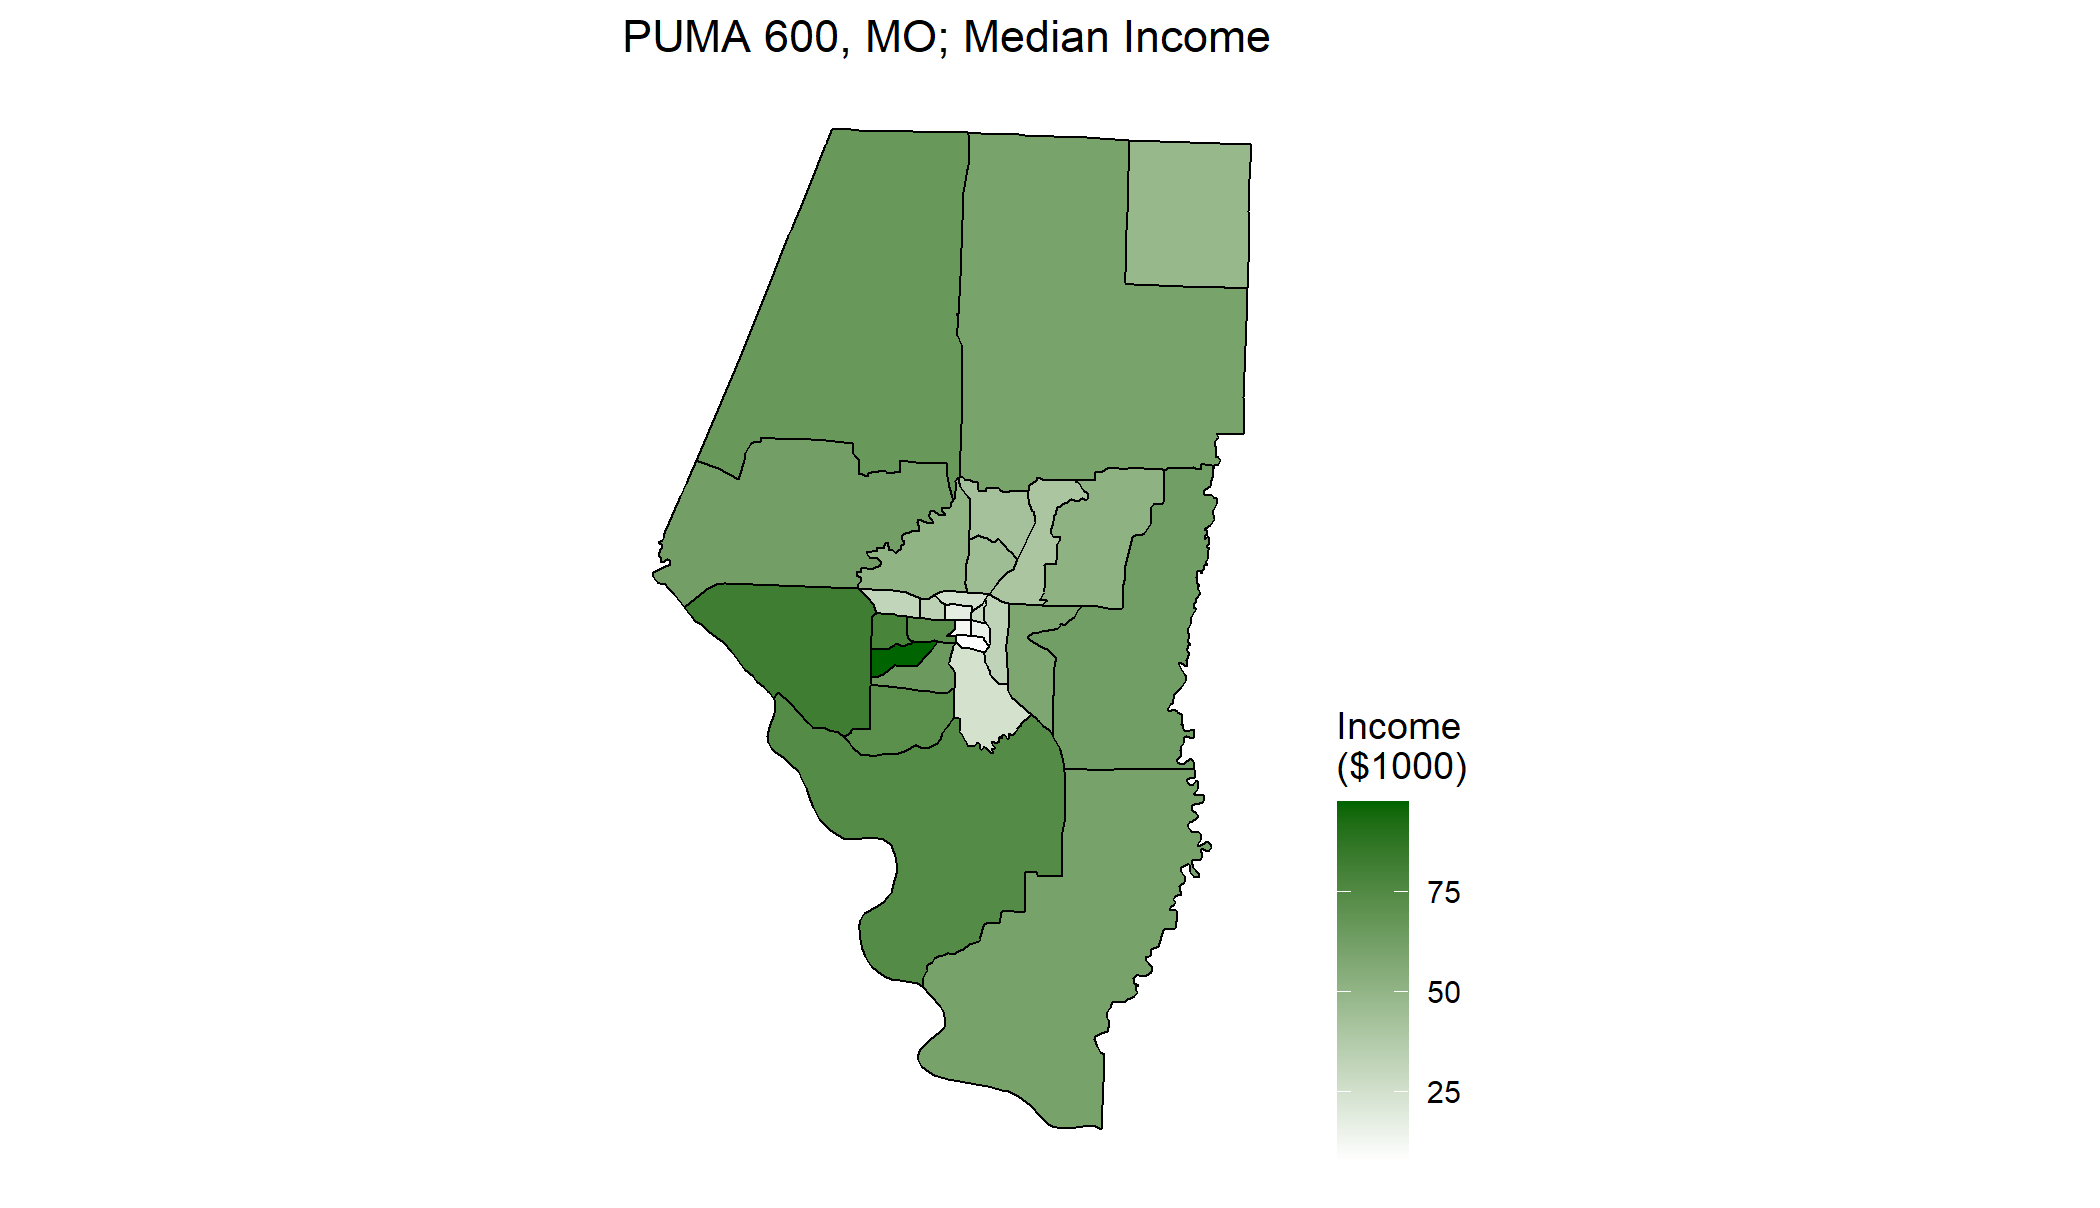
\includegraphics[scale = 0.9]{median_mo_map_big.png}
\caption{An example PUMA with nested tracts: PUMA 600 (Boone County) in MO. Tracts are shaded according to 2015 ACS 5-year estimates of median household income.}
\label{fig:boonepuma}
\end{figure}

\begin{figure}
\centering
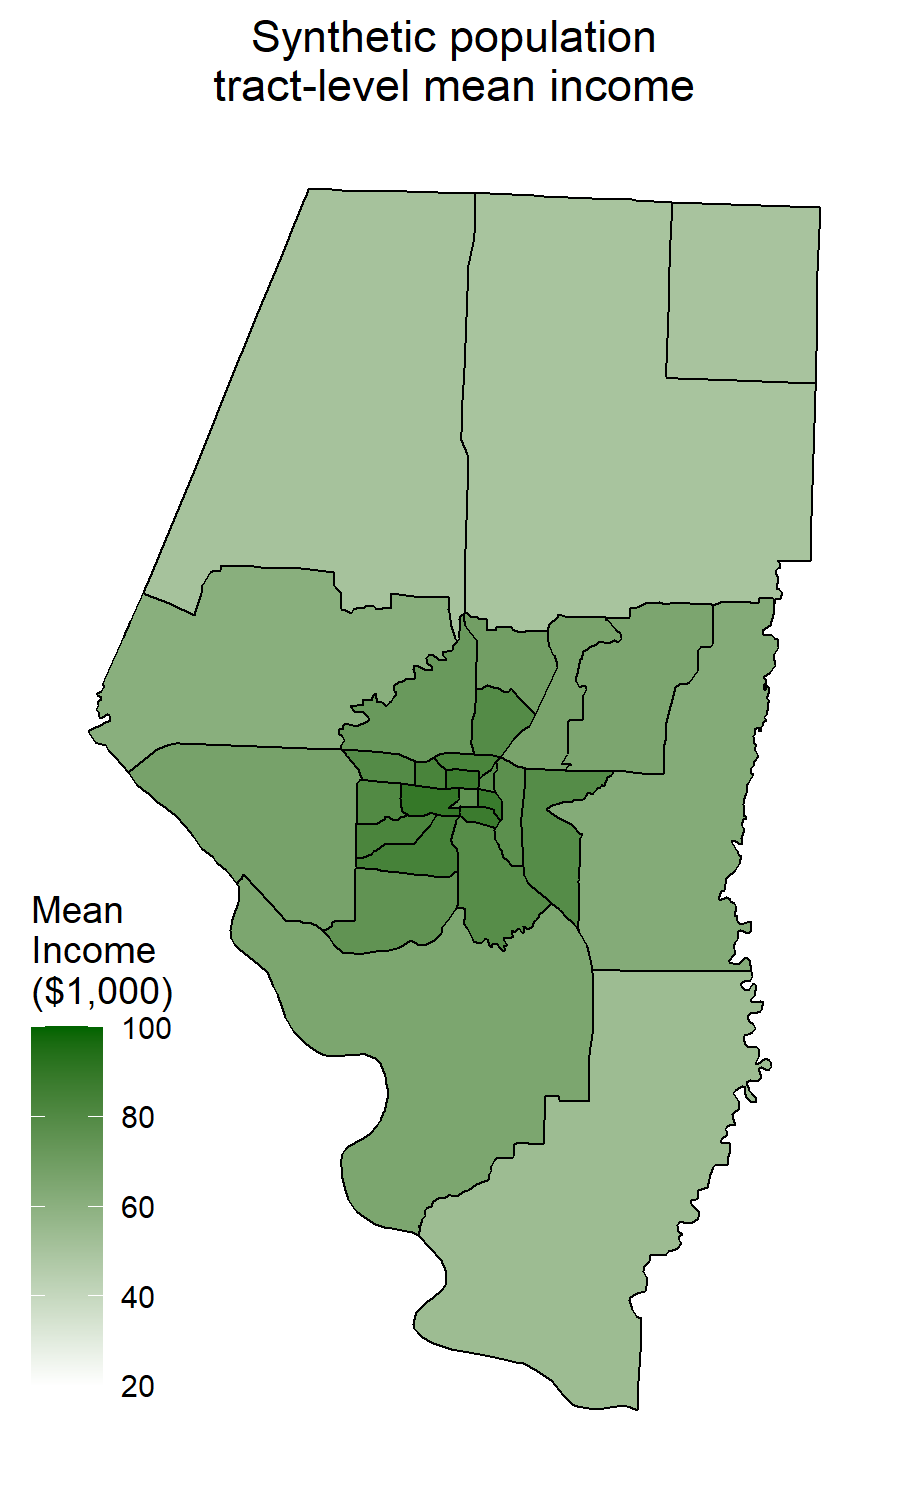
\includegraphics[width = 0.3\textwidth]{mean.png}
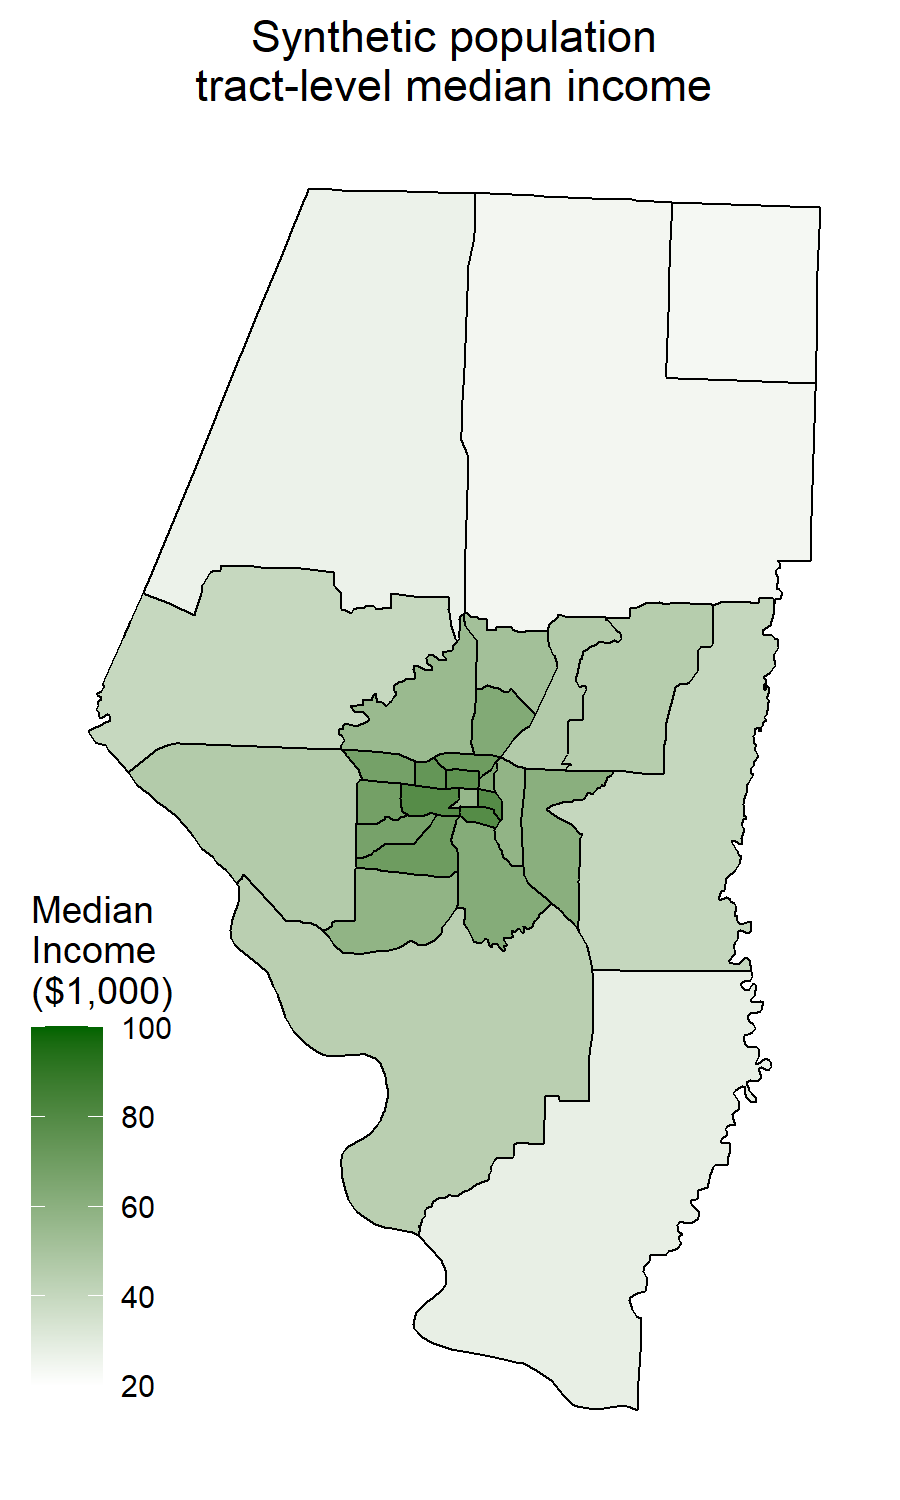
\includegraphics[width = 0.3\textwidth]{median.png}
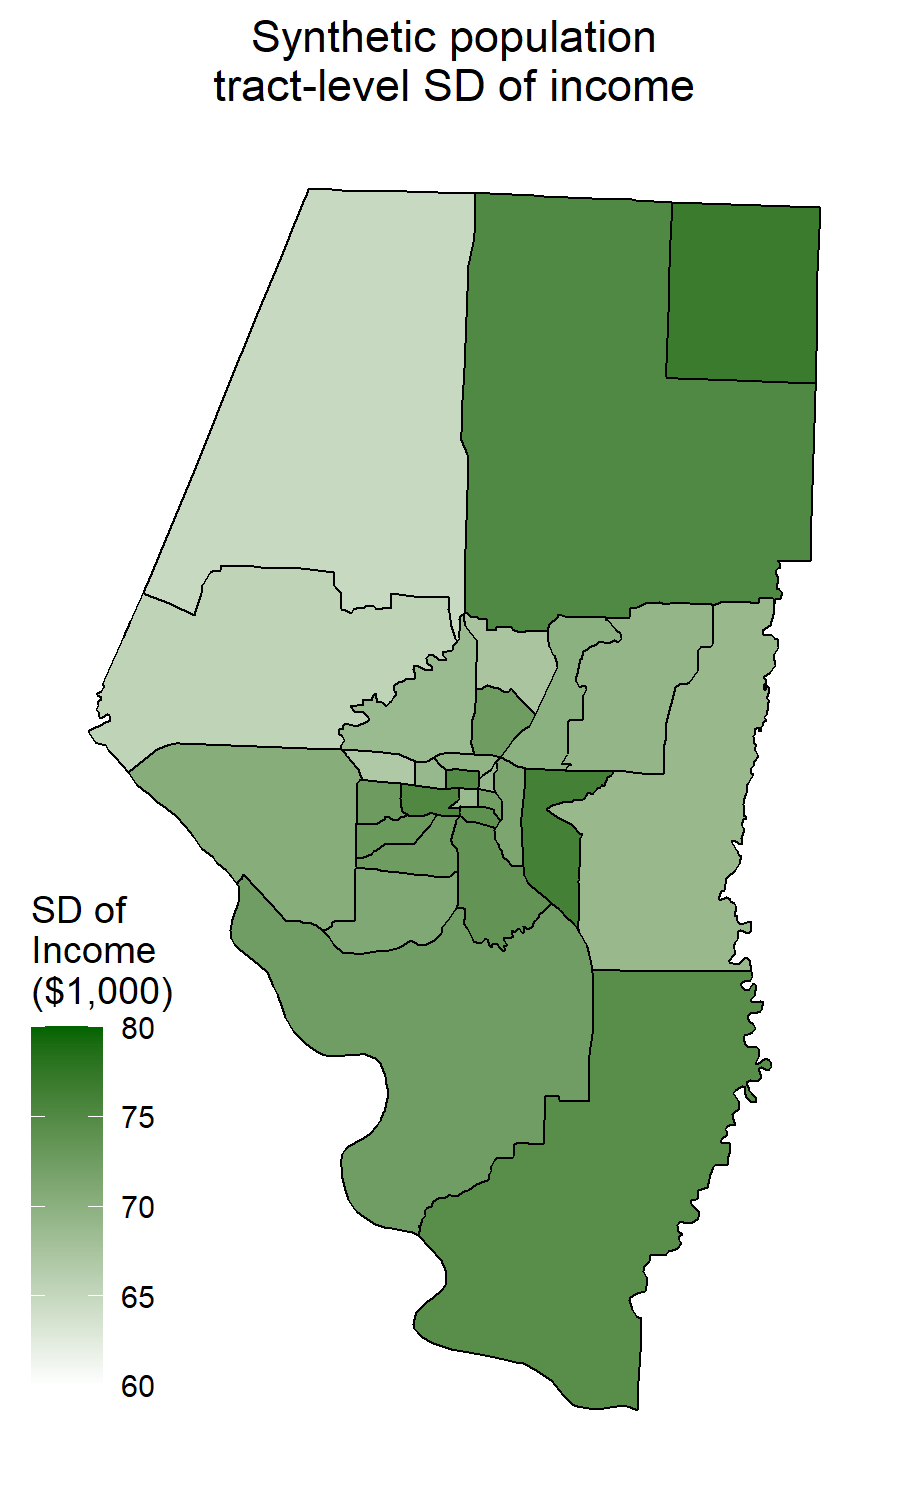
\includegraphics[width = 0.3\textwidth]{sd.png}
\caption{True tract-level means, medians, and standard deviations of income for the synthetic population. The first two exhibit a noticeable inside-out spatial pattern, while the third is a bit different but still appears to have spatial dependence.}
\label{fig:pops}
\end{figure}

\begin{figure}
  \centering
  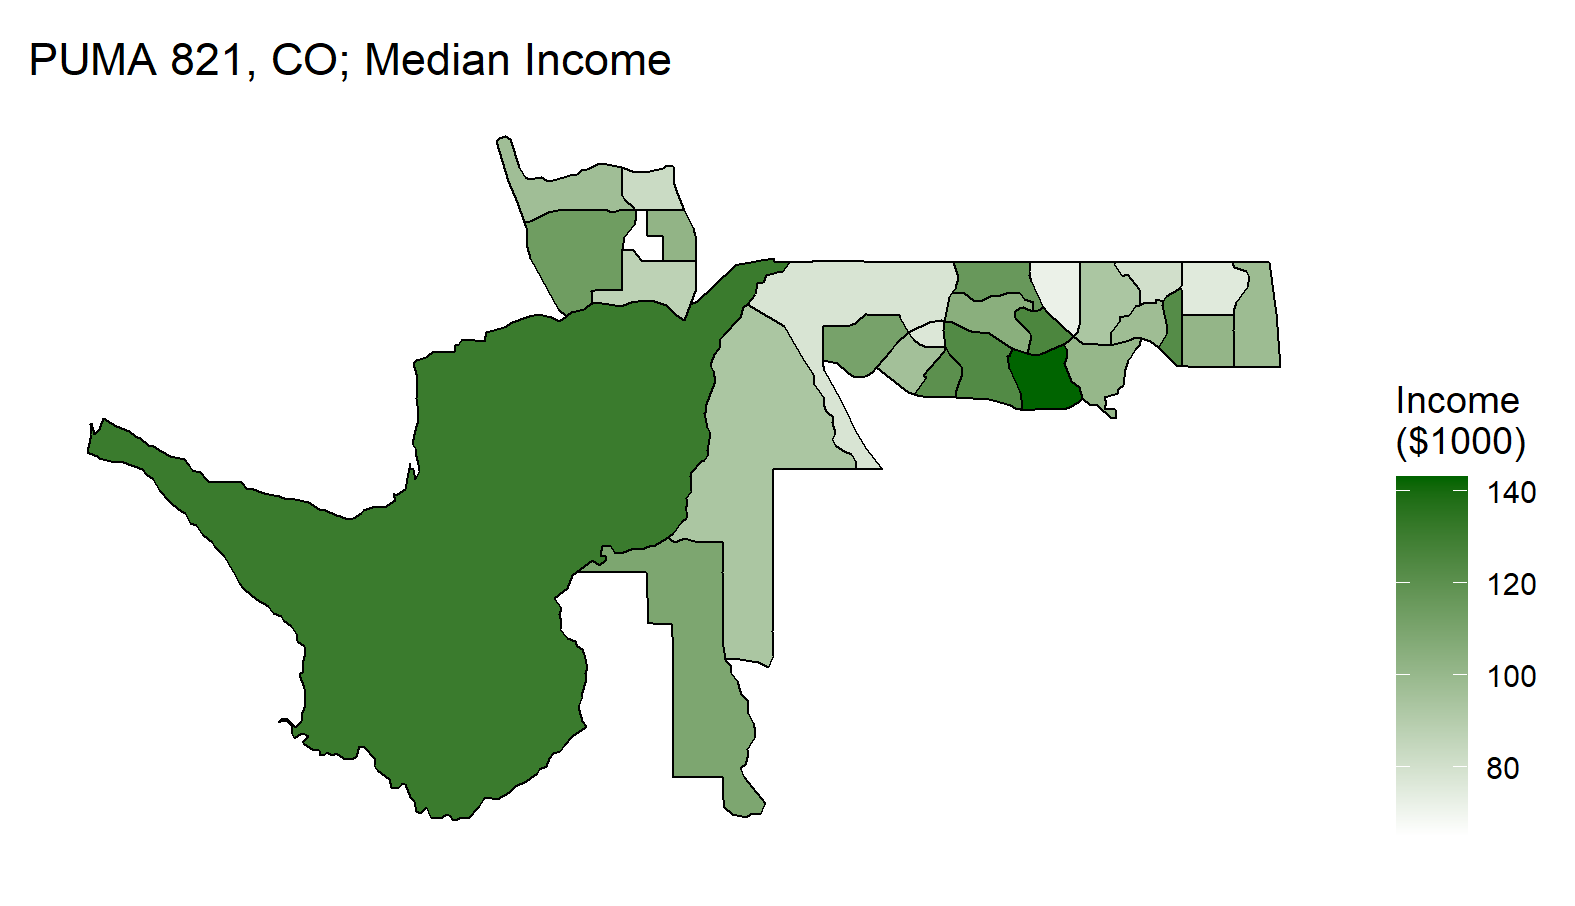
\includegraphics[width = 0.45\textwidth]{median_co_map.png}
  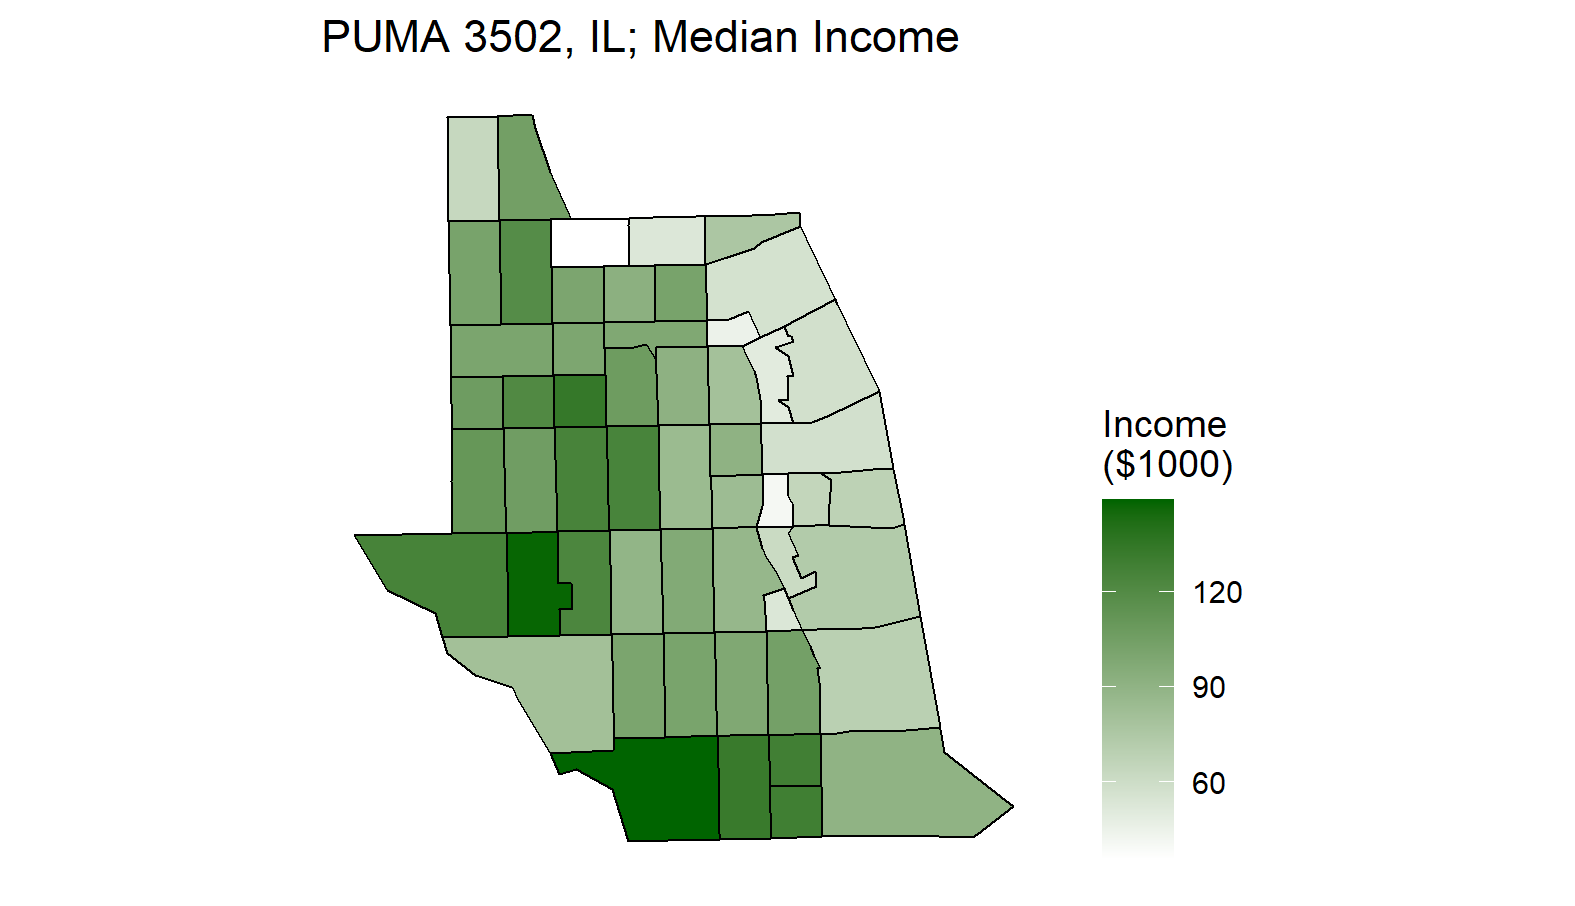
\includegraphics[width = 0.45\textwidth]{median_il_map.png}
  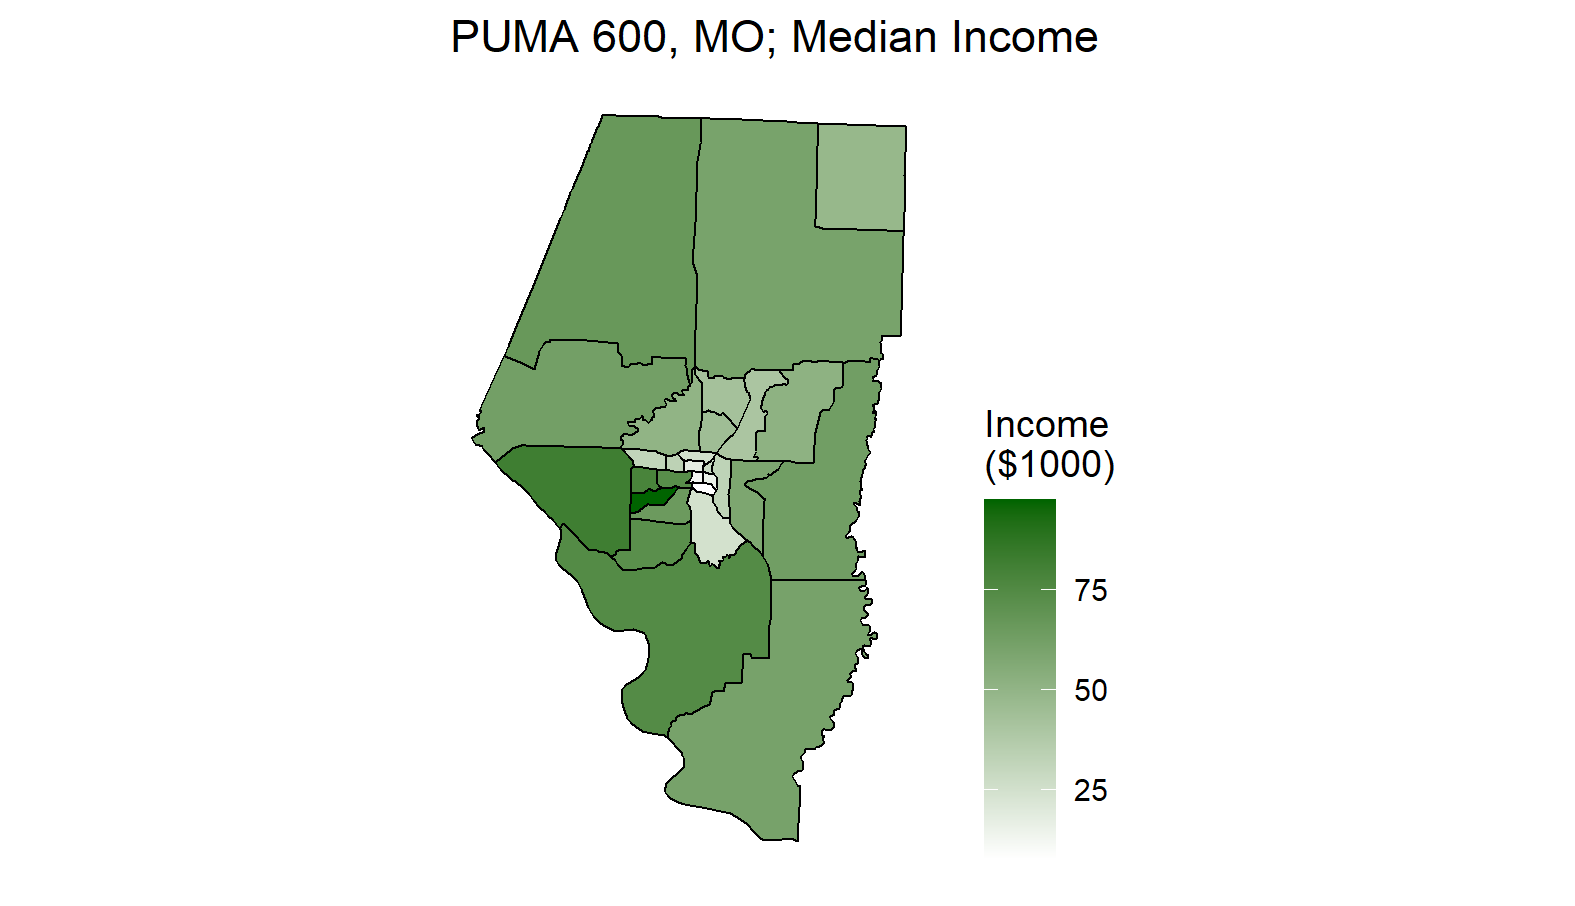
\includegraphics[width = 0.45\textwidth]{median_mo_map.png}
  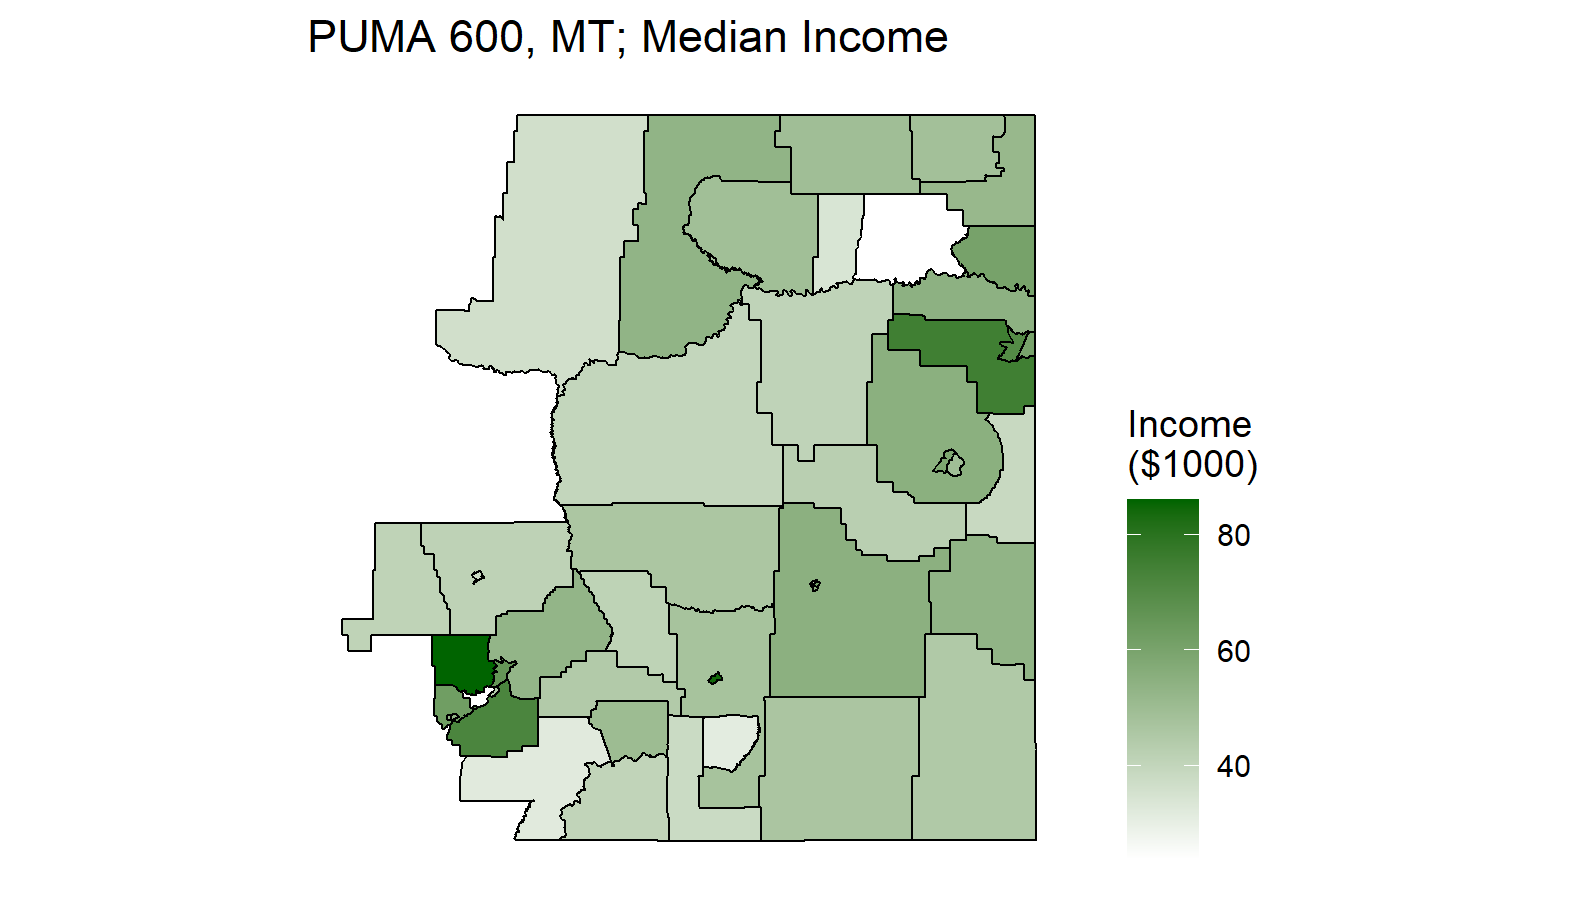
\includegraphics[width = 0.45\textwidth]{median_mt_map.png}
  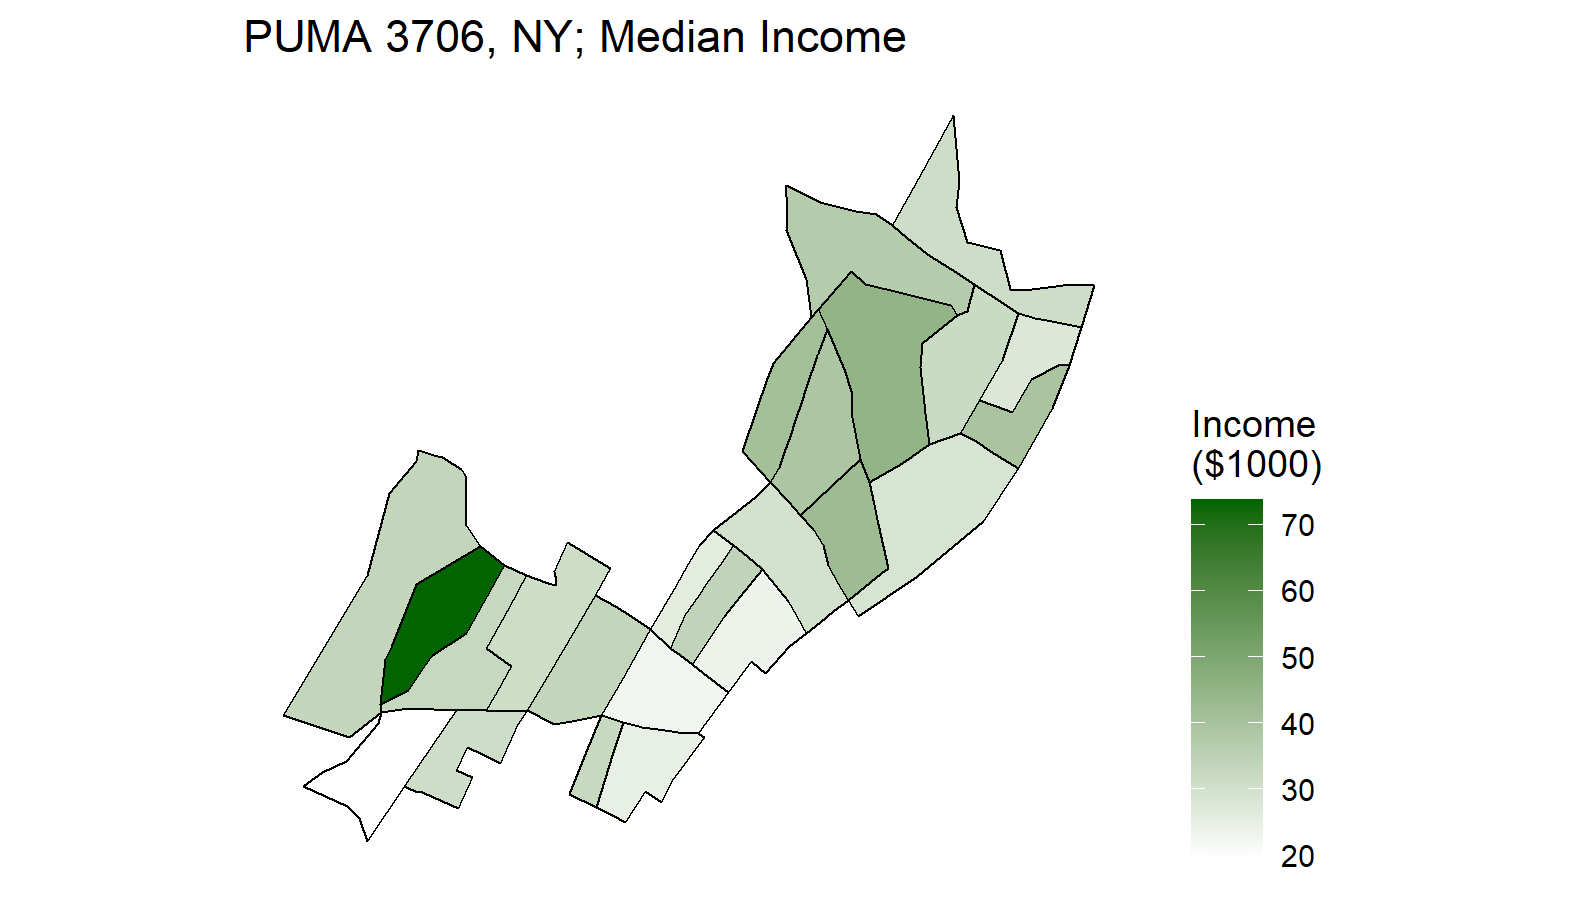
\includegraphics[width = 0.45\textwidth]{median_ny_map.png}
  \caption{Maps of each PUMA used in the main text with each of the census tracts. Each tract within each PUMA is shaded according to the 2015 ACS 5-year period estimate of median household income.}
  \label{fig:allpumas.median}
\end{figure}

\clearpage

\section{LATENT PRLN DENSITY FUNCTIONALS}\label{app:functionals}
\setcounter{table}{0}
The latent PRLN density is given by
\begin{align*}
\pi(x) = \sum_{k=1}^Kp_kf_k(x).
\end{align*}
Let $k^*$ denote the largest knot which is less than an available estimate of the median. Then
\begin{align*}
  f_k(x) = &\  \frac{1}{\kappa_{k+1} - \kappa_k} \times \mathbbm{1}(\kappa_k < x \leq \kappa_{k+1}) && \mbox{ if $k^* \leq k^*$ },\nonumber\\
  = &\  \frac{\alpha_k\kappa_k^{\alpha_k}x^{-\alpha_k - 1}}{1 - \left(\frac{\kappa_k}{\kappa_{k+1}}\right)^{\alpha_k}} \times \mathbbm{1}(\kappa_k < x \leq \kappa_{k+1}) && \mbox{ if $k^* < k < K$ },\nonumber\\
  = &\  \alpha_k\kappa_kx^{-\alpha_k - 1} \times \mathbbm{1}(\kappa_K < x) && \mbox{ if $k = K$ }.
\end{align*}
For the $k$th bin, let $\mu_k$ denote its mean, $\sigma^2_k$ denote its variance, $F_k(x)$ denote its CDF, and $F^{-1}_k$ denote its quantile function, and $I_k$ denote its integrated Lorenz curve. Then the following sections derive formulas for several functionals in terms of these basic building blocks. 
\subsection{Mean}
Let $\mu = \E_\pi[x]$. Then
\begin{align*}
\mu = \sum_{k=1}^Kp_k\mu_k.
\end{align*}
Note that this requires that each $\mu_k$ exist.
\subsection{Variance}
Let $\sigma^2 = \var_{\pi}[x]$. Then the conditional variance formula yields
\begin{align*}
  \sigma^2 = \sum_{k=1}^Kp_k\sigma_k^2 + \sum_{k=1}^Kp_k(\mu_k - \mu)^2.
\end{align*}
Note that this requires that each $\sigma_k^2$ exist.
\subsection{CDF}
Let $\Pi(x)$ denote the CDF corresponding to $\pi(x)$. Then
\begin{align*}
  \Pi(x) = \begin{cases}
    0, & \mbox{ if } x \leq \kappa_1\\
    F_1(x), & \mbox{ if } \kappa_1 < x \leq \kappa_2\\
    p_1 + p_2*F_2(x), & \mbox{ if } \kappa_2 < x \leq \kappa_3 \\
  \vdots  & \vdots  \\
    \sum_{k=1}^{j-1}p_k + p_jF_j(x), &\mbox{ if } \kappa_j < x \leq \kappa_{j+1}\\
   \vdots & \vdots  \\
    \sum_{k=1}^{K-1}p_k + p_KF_K(x), &\mbox{ if } \kappa_{K} < x  \leq \kappa_{K+1} \\
    1, & \mbox{ if } \kappa_{K+1} \leq x.
  \end{cases}
\end{align*}
Note that bin probabilities are given by a difference in the CDF evaluated at two knots, i.e.
\begin{align*}
p_k = \Pi(\kappa_k) - \Pi(\kappa_{k-1}).
\end{align*}
\subsection{Quantile function}
Let $\Pi^{-1}$ denote the quantile function associated with $\pi(x)$. Then
\begin{align*}
  \Pi^{-1}(\tau) = \begin{cases}
    F^{-1}_1\left(\frac{\tau}{p_1}\right), & \mbox{ if } 0 \leq \tau \leq p_1 \\
    F^{-1}_2\left(\frac{\tau - p_1}{p_2}\right), & \mbox{ if } p_1 < \tau \leq p_1 + p_2 \\
  \vdots  & \vdots \\
    F^{-1}_j\left(\frac{\tau - \sum_{k=1}^{j-1}p_k}{p_j}\right), & \mbox{ if } \sum_{k=1}^{j-1}p_{k} < \tau \leq \sum_{k=1}^jp_{k} \\
  \vdots  & \vdots \\
    F^{-1}_K\left(\frac{\tau - \sum_{k=1}^{K-1}p_k}{p_K}\right), & \mbox{ if } \sum_{k=1}^{K-1}p_{k} < \tau \leq 1.
  \end{cases}
\end{align*}
Note that $\Pi^{-1}$ is not everywhere differentiable as a function of the $p_k$s.

\subsection{Integrated Lorenz curve}
The Lorenz curve for a PDF $f$ with associated CDF $F$ and mean $\mu$ is defined as
\begin{align*}
  L(\tau) = \frac{1}{\mu}\int_{-\infty}^{F^{-1}(\tau)}y f(y) dy.
\end{align*}
The integrated Lorenz curve is given by
\begin{align*}
I = \int_0^1L(\tau)d\tau = \int_{-\infty}^{\infty}L[F(x)]f(x)dx.
\end{align*}
Let $L_k$ denote the Lorenz curve for the $k$th bin. Let $\kappa_{k^*}$ denote the largest knot such that $\kappa_{k^*} \leq x = \Pi^{-1}(\tau)$ and note that for any Lorenz curve $L(0)=0$ and $L(1)=1$.  Then we can express the Lorenz curve for the latent PRLN density as
\begin{align*}
  L[\Pi(x)] & = \frac{1}{\mu}\int_{-\infty}^x y \pi(y) dy \\
          & = \frac{1}{\mu}\left[\sum_{j=1}^{k^*-1}p_j\mu_j + p_{k^*}\int_{\kappa_{k^*}}^xyf_{k^*}(y)dy\right] \\
          & = \frac{1}{\mu}\left[\sum_{j=1}^{k^*-1}p_j\mu_j + p_{k^*}\mu_{k^*}L_{k^*}[F_{k^*}(x)]\right] \\
          & = \frac{1}{\mu}\sum_{k=1}^Kp_k\mu_kL_k[F_k(x)].
\end{align*}
This implies that if we state the Lorenz curve in its original form as a pure function of $\tau$, we have
\begin{align*}
L(\tau) = \frac{1}{\mu}\sum_{k=1}^Kp_k\mu_kL_k\{F_k[F^{-1}(\tau)]\}.
\end{align*}
Then the integrated Lorenz curve can be written as
\begin{align*}
  I & = \frac{1}{\mu}\sum_{k=1}^Kp_k\mu_k\int_{-\infty}^{\infty}L_k[F_k(x)]\pi(x)dx \\
  & = \frac{1}{\mu}\sum_{k=1}^Kp_k\mu_k\sum_{j=1}^Kp_j\int_{\kappa_j}^{\kappa_{j+1}}L_k[F_k(x)]f_j(x)dx \\
    & = \frac{1}{\mu}\sum_{k=1}^Kp_k\mu_k\left[p_k\int_{\kappa_{k}}^{\kappa_{k+1}}L_k[F_k(x)]f_k(x)dx + \sum_{j=k+1}^Kp_j\right] \\
    & = \frac{1}{\mu}\sum_{k=1}^{K}p_k\mu_k\left[p_kI_k + \sum_{j=k+1}^Kp_j\right].
\end{align*}

\subsection{Distribution shares}
The Lorenz curve represents the proportion of aggregate income that goes to the lower $p$ proportion of the income distribution, for any $0 < p < 1$. So for an income distribution, distribution shares (income shares) are given by differences in the Lorenz curve evaluated at two points. For $0\leq \tau_1 < \tau_2 \leq1$ the aggregate income that goes to the distribution between $\tau_1$ and $\tau_2$ is given by
\begin{align*}
s(\tau_1, \tau_2) = L(\tau_2) - L(\tau_1).
\end{align*}
\subsection{Gini index}
The Gini index for a continuous distribution can be expressed in terms of the Lorenz curve as
\begin{align*}
G = 1 - 2\int_0^1L(\tau)d\tau = 1 - 2I
\end{align*}

\subsection{Applying to the latent PRLN density}
To apply this to the latent PRLN density, we need to find all of the building blocks for each bin type: uniform, truncated Pareto, and Pareto distributed.

\subsubsection{Uniform bins}
For uniform bins:
\begin{align*}
  \mu_k & = \frac{1}{2}(\kappa_{k+1} + \kappa_k) &&&\\
  \sigma_k^2 &= \frac{1}{12}(\kappa_{k+1} - \kappa_k)^2 &&&\\
  F_k(x) &= \frac{x - \kappa_k}{\kappa_{k+1} - \kappa_k} &&& \mbox{ for } \kappa_k \leq x \leq \kappa_{k+1} \\
  F^{-1}_k(\tau) & = \kappa_k + \tau (\kappa_{k + 1} - \kappa_k). &&&
\end{align*}
Then the Lorenz curve is
\begin{align*}
  L_k[F_k(x)] &= \frac{1}{\mu_k}\int_{\kappa_k}^x y f_k(y) dy \\
              &= \frac{1}{2\mu_k}\frac{x^2 - \kappa_k^2}{\kappa_{k+1} - \kappa_k}.
\end{align*}
The integrated Lorenz curve is
\begin{align*}
  I_k & = \int_{\kappa_k}^{\kappa_{k+1}}\frac{1}{2\mu_k}\frac{x^2 - \kappa_k^2}{(\kappa_{k+1} - \kappa_k)^2}dx \\
      & = \frac{1}{2\mu_k(\kappa_{k+1} - \kappa_k)^2}\left[\frac{\kappa_{k+1}^3}{3} - \frac{\kappa_{k}^3}{3} - (\kappa_{k+1} - \kappa_k)\kappa_k^2\right]\\
      & = \frac{1}{\mu_k}\left[\frac{(\kappa_{k+1} - \kappa_k)(\kappa_{k+1}^2 + \kappa_{k+1}\kappa_k + \kappa_k^2)}{6(\kappa_{k+1} - \kappa_k)^2} - \frac{\kappa_{k}^2}{2(\kappa_{k+1}-\kappa_k)}\right] \\
      & = \frac{1}{\mu_k}\frac{\kappa_{k+1}^2 + \kappa_{k+1}\kappa_{k} + \kappa_k^2 - 3 \kappa_k^2}{6(\kappa_{k+1} - \kappa_k)} \\
      & = \frac{\kappa_{k+1} + 2\kappa_k}{6\mu_k}\\
      & = \frac{\kappa_{k+1} + 2\kappa_k}{3(\kappa_{k+1} + \kappa_k)}\\
      & = \frac{1}{3}\left(1 + \frac{\kappa_k}{\kappa_k + \kappa_{k+1}}\right).
\end{align*}

\subsubsection{Pareto bins}
For Pareto distributed bins
\begin{align*}
  \mu_K & = \frac{\alpha_K\kappa_K}{\alpha_K - 1} &&& \mbox{ if } \alpha_K > 1\\
  \sigma_K^2 &= \frac{\kappa_K^2\alpha_K}{(\alpha_K-1)^2(\alpha_K-2)} &&& \mbox{ if } \alpha_K > 2\\
  F_K(x) &= 1 - \left(\frac{\kappa_K}{x}\right)^{\alpha_K} &&& \mbox{ for } \kappa_K \leq x \\
  F^{-1}_K(\tau) & = \frac{\kappa_K}{(1 - \tau)^{1/\alpha_K}}. &&&
\end{align*}
Then the Lorenz curve is given by
\begin{align*}
  L_K[F_K(x)] & = \frac{1}{\mu_K}\int_{\kappa_K}^{x} \alpha_K\kappa_K^{\alpha_K} y^{-\alpha_K} dy \\
              & = \frac{\alpha_K\kappa_K^{\alpha_K}}{\mu_K}\left(-\frac{1}{\alpha_K - 1}y^{-\alpha_K + 1}\right)_{\kappa_K}^{x} \\
              & = \frac{1}{\mu_K}\frac{\alpha_K}{\alpha_K - 1}\left(\kappa_K - \kappa_K^{\alpha_K}x^{1 - \alpha_K}\right).
\end{align*}
Then the integrated Lorenz curve is
\begin{align*}
  I_K & = \int_{\kappa_K}^{\infty}L_K[F_K(x)]f_K(x) dx\\
      & = \frac{1}{\mu_k}\frac{\alpha_K}{\alpha_K - 1}\left(\kappa_K - \kappa_{K}^{\alpha_K}\int_{\kappa_K}^{\infty}x^{1 - \alpha_K}\alpha_K\kappa_K^{\alpha_K}x^{-\alpha_K - 1} dx\right) \\
        & = \frac{1}{\mu_k}\frac{\alpha_K}{\alpha_K - 1}\left(\kappa_K - \frac{1}{2}\int_{\kappa_K}^{\infty}2\alpha_K\kappa_K^{2\alpha_K}x^{-2\alpha_K} dx\right) \\
      & = \frac{1}{\mu_K}\frac{\alpha_K}{\alpha_K - 1}\left(\kappa_K - \frac{1}{2}\frac{2\alpha_K}{2\alpha_K - 1}\kappa_K\right)\\
      & = 1 - \frac{\alpha_K}{2\alpha_K - 1}.
\end{align*}

\subsubsection{Truncated Pareto bins}
For truncated Pareto bins
\begin{align*}
  \mu_k & = \frac{\alpha_k\kappa_k}{\alpha_k - 1}\frac{1 - \left(\frac{\kappa_k}{\kappa_{k+1}}\right)^{\alpha_k - 1}}{1 - \left(\frac{\kappa_k}{\kappa_{k+1}}\right)^{\alpha_k}} &&& \mbox{ if } \alpha_k > 1\\
  \sigma_k^2 &= \frac{\alpha_k}{\alpha_k - 2}\kappa_k^2\frac{1 - \left(\frac{\kappa_k}{\kappa_{k+1}}\right)^{\alpha_k - 2}}{1 - \left(\frac{\kappa_k}{\kappa_{k+1}}\right)^{\alpha_k}} - \frac{\alpha_k^2}{(\alpha_k-1)^2}\kappa_k^2\frac{\left[1 - \left(\frac{\kappa_k}{\kappa_{k+1}}\right)^{\alpha_k - 1}\right]^2}{\left[1 - \left(\frac{\kappa_k}{\kappa_{k+1}}\right)^{\alpha_k }\right]^2} &&& \mbox{ if } \alpha_k > 2\\
  F_k(x) &= \frac{1 - \left(\frac{\kappa_k}{x}\right)^{\alpha_k}}{1 - \left(\frac{\kappa_k}{\kappa_{k+1}}\right)^{\alpha_k}} &&& \mbox{ for } \kappa_k \leq x \leq \kappa_{k+1} \\
  F^{-1}_k(\tau) & = \frac{\kappa_k}{\left\{1 - \tau\left[1 - \left(\frac{\kappa_k}{\kappa_{k+1}}\right)^{\alpha_k}\right]\right\}^{1/\alpha_k}}. &&&
\end{align*}
The formulas for means and variances can be extended to $\alpha_k > 0$ so long as care is taken to account for special cases when $\alpha_k = 1$ and $\alpha_k = 2$.

Next, the Lorenz curve is given by
\begin{align*}
  L_k[F_k(x)] & = \frac{1}{\mu_k}\int_{\kappa_k}^{x} \frac{\alpha_k\kappa_k^{\alpha_k} y^{-\alpha_k}}{1 - \left(\frac{\kappa_k}{\kappa_{k+1}}\right)^{\alpha_k}} dy  \\
              & = \frac{1}{\mu_k}\frac{\alpha_k\kappa_k^{\alpha_k}}{1 - \left(\frac{\kappa_k}{\kappa_{k+1}}\right)^{\alpha_k}}\left[-\frac{1}{\alpha_k - 1}(x^{1 - \alpha_k} - \kappa_k^{1 - \alpha_k})\right] \\
              & = \frac{1}{\mu_k}\frac{\alpha_k}{\alpha_k - 1}\frac{\kappa_k^{\alpha_k}}{1 - \left(\frac{\kappa_k}{\kappa_{k+1}}\right)^{\alpha_k}}\left[\kappa_k^{1-\alpha_k} - x^{1 - \alpha_k}\right]\\
              & = \frac{\kappa_k}{\mu_k}\frac{\alpha_k}{\alpha_k - 1}\frac{1 - \left(\frac{\kappa_k}{x}\right)^{\alpha_k - 1}}{1 - \left(\frac{\kappa_k}{\kappa_{k+1}}\right)^{\alpha_k}}.
\end{align*}
Then the integrated Lorenz curve is given by
\begin{align*}
  I_k & = \int_{\kappa_k}^{\kappa_{k+1}}L_k[F_k(x)]f_k(x)dx \\
      & = \frac{1}{\mu_k}\frac{\alpha_k}{\alpha_k - 1}\frac{\kappa_k^{\alpha_k}}{1 - \left(\frac{\kappa_k}{\kappa_{k+1}}\right)^{\alpha_k}}\int_{\kappa_k}^{\kappa_{k+1}}\left[\kappa_k^{1-\alpha_k} - x^{1 - \alpha_k}\right]\frac{\alpha_k\kappa_k^{\alpha_k}}{1 - \left(\frac{\kappa_k}{\kappa_{k+1}}\right)^{\alpha_k}}x^{-\alpha_k - 1}dx \\
      & = \frac{1}{\mu_k}\frac{\alpha_k}{\alpha_k - 1}\frac{1}{1 - \left(\frac{\kappa_k}{\kappa_{k+1}}\right)^{\alpha_k}}\left[\kappa_k - \frac{1}{2}\frac{1 - \left(\frac{\kappa_k}{\kappa_{k+1}}\right)^{2\alpha_k}}{1 - \left(\frac{\kappa_k}{\kappa_{k+1}}\right)^{\alpha_k}}\int_{\kappa_k}^{\kappa_{k+1}}\frac{2\alpha_k\kappa_k^{2\alpha_k}}{1 - \left(\frac{\kappa_k}{\kappa_{k+1}}\right)^{2\alpha_k}}x^{-2\alpha_k}dx\right] \\
      & = \frac{1}{\mu_k}\frac{\alpha_k}{\alpha_k - 1}\frac{1}{1 - \left(\frac{\kappa_k}{\kappa_{k+1}}\right)^{\alpha_k}}\left[\kappa_k - \frac{1}{2}\frac{1 - \left(\frac{\kappa_k}{\kappa_{k+1}}\right)^{2\alpha_k}}{1 - \left(\frac{\kappa_k}{\kappa_{k+1}}\right)^{\alpha_k}}\frac{2\alpha_k}{2\alpha_k - 1}\kappa_k\frac{1 - \left(\frac{\kappa_k}{\kappa_{k+1}}\right)^{2\alpha_k - 1}}{1 - \left(\frac{\kappa_k}{\kappa_{k+1}}\right)^{2\alpha_k}}\right] \\
      & = \frac{\kappa_k}{\mu_k}\frac{\alpha_k}{\alpha_k - 1}\frac{1}{1 - \left(\frac{\kappa_k}{\kappa_{k+1}}\right)^{\alpha_k}}\left[1 - \frac{1 - \left(\frac{\kappa_k}{\kappa_{k+1}}\right)^{2\alpha_k - 1}}{1 - \left(\frac{\kappa_k}{\kappa_{k+1}}\right)^{\alpha_k}}\frac{\alpha_k}{2\alpha_k - 1}\right] \\
      & = 1 - \frac{\alpha_k}{2\alpha_k - 1}\frac{1 - \left(\frac{\kappa_k}{\kappa_{k+1}}\right)^{2\alpha_k - 1}}{1 - \left(\frac{\kappa_k}{\kappa_{k+1}}\right)^{\alpha_k}}\\
      & = 1 - \frac{\alpha_k\kappa_{k+1}^{1 - \alpha_k}}{2\alpha_k - 1}\frac{\kappa_{k+1}^{2\alpha_k - 1} - \kappa_k^{2\alpha_k - 1}}{\kappa_{k+1}^{\alpha_k} - \kappa_k^{\alpha_k}}.
\end{align*}

\section{GENERATING THE SYNTHETIC POPULATION}\label{app:synpop}
\setcounter{table}{0}
We construct the population in our simulation study to have the same number of households per tract as the 2014 ACS 5-year period estimates of household population for the Boone County, MO PUMA. We then divide the population into the same 106 strata that exist in the 2014 Boone County 5-year PUMS -- a stratum is defined as all observations with the same survey weight. The population of each stratum is assumed to be to $n_sw_s$ where $n_s$ is the sample size of stratum $s$ in the PUMS, and $w_s$ is the survey weight associated with stratum $s$. To fully specify the population we need to know number of households in each tract/stratum combination, though in reality this is unknown. Nevertheless, we know that the PUMS strata are based in part on census tracts \citep{acs2015}, so in our synthetic population we assign the households in a given stratum to a small number of tracts using an algorithm that produces tract and stratum assignments that are closely related.

Next, an income is generated for each household using a two-component mixture of lognormals with parameters that depend on both their tract and stratum. The resulting tract-level distributions are mixtures of lognormals. Figure~\ref{fig:pops} in the Supplementary Materials contains maps of the true tract-level means, medians, and standard deviations of income for the synthetic population.

The above description omits two important pieces of how the population is generated. First, how strata are assigned to tracts, and second, how incomes are generated for each tract/stratum combination. We take these in turn.

\subsection{Assigning strata to tracts}
Algorithm~\ref{alg:stratum2tract} describes how strata are assigned to tracts. Essentially, for each tract, we randomly select a stratum, then assign as much of that stratum as we can to the tract. If the stratum fully fits in the tract (along with the strata already assigned to it), then the stratum is deleted from the pool of available strata, and a new one is randomly selected to repeat the process. If the stratum does not fit, then the stratum is returned to the pool of available strata with its remaining population, and we move on to the next tract.
\begin{algorithm}[ht]
  \begin{algorithmic}
  \item
    \FORALL{tract}
    \STATE{Initialize tract.pop = 0}
    \WHILE{tract.pop $<$ tract.popest}
    \STATE{Randomly select a stratum with stratum.pop $>$ 0}
    \STATE{Set P $=$ MIN(stratum.pop, tract.popest - tract.pop)}
    \STATE{Assign P  members of the stratum to tract}
    \STATE{Set target.pop $+=$ P}
    \STATE{Set stratum.pop $-=$ P}
    \ENDWHILE
    \ENDFOR
  \end{algorithmic}
  \caption{Assign strata to tracts. Assume that tract.popest is the desired population of the tract, and that stratum.pop is initialized with the assigned population of the stratum.}
  \label{alg:stratum2tract}
\end{algorithm}

\subsection{Generating incomes for tract/stratum combinations}
Generating the incomes is more complex. For each tract/stratum combination we define a two-component mixture of lognormal distributions, using the PUMS data as a guide. To do this, we need several intermediate quantities. First, using the PUMS data, let $\widehat{m}$ denote the sample mean of $z = \log(\mathrm{income} + 1)$ and let $\widehat{s}$ denote the sample standard deviation. We use the offset of one because there are incomes equal to zero in the dataset.

Next for each stratum, we compute the a measure of dispersion of $z$ and a measure of how far $z$ tends to be away from the the PUMA mean. Let $i=1,2,\dots,n_s$ index observations in stratum $s$, and $z_{is}$ denote log offset income for each of those observations, as in the previous paragraph. Then define
\begin{align*}
D_s = \frac{1}{n_s + 5}\sum_{i=1}^{n_s}(z_{is} - \widehat{m}).
\end{align*}
This is a measure of how far the stratum tends to be from the PUMA average, regularized toward zero since many strata have as few as one observation. Similarly, define
\begin{align*}
H_s^2 = \frac{n_s}{n_s + 500}\frac{1}{n_s}\sum_{i=1}^{n_s}(z_{is} - \overline{z}_s)^2 + \frac{500}{n_s + 500}\widehat{s}^2,
\end{align*}
where $\overline{z}_s$ is the mean of $z_{is}$ in stratum $s$. This is a measure of dispersion in the stratum, again regularized to be much closer the PUMA level dispersion. Note that we divide by $n_s$ instead $n_s - 1$ to avoid dividing by zero in strata with only one member.

Finally, we need a tract-level and a stratum-level covariate to use these quantities with. For a tract $r$, let $\mathrm{dist}_r$ denote the average distance of tract $r$ from the center of the bounding box containing the PUMA, and let $ \mathrm{sdist}_r = (\mathrm{dist}_r - \mathrm{mean}(\mathrm{dist}_{1:R}))/\mathrm{sd}(\mathrm{dist}_{1:R})$ denote the scaled distance from the center for $r$. Next let $w_s$ denote the unique weight associated with stratum $s$. Finally let $W_s = (\log w_s - \mathrm{mean}(\log w_{1:S})) / \mathrm{sd}(\log w_{1:S})$ denote the scaled log weight for $s$.

Using these quantities, we need to choose the mean parameters $\mu_1$ and $\mu_2$, the standard deviation parameters $\sigma_1$ and $\sigma_2$, and the mixture weight $\omega$, all for a given tract/stratum combination $(r,s)$. We use the following quantities:
\begin{align*}
  \omega &= \frac{1}{1 + \exp[0.2 \mathrm{sdist}_r + 0.2 * W_s]}\\
  \mu_1 &= 0.87\widehat{m} - 0.3 \mathrm{sdist}_r + D_s\\
  \mu_2 &= 1.05\widehat{m} - 0.2 \mathrm{sdist}_r + 1.5 D_s\\
  \sigma_1 & = \exp\left[\frac{\mathrm{sdist}_r}{5} - \frac{\log H_s}{5}\right]\\
  \sigma_2 & = 0.6\exp\left[\frac{\mathrm{sdist}_r}{5} - \frac{\log H_s - \log 0.6}{5}\right].
\end{align*}
We arrived at these settings through exploratory analysis until we found a population of incomes that looked somewhat like a real income distribution. The distribution includes natural spatial variation across tracts and variation across strata, in an attempt to mimic the observed data.

\clearpage

\section{EVALUATING POINT ESTIMATES}\label{app:acstab}
\setcounter{table}{0}
  % latex table generated in R 3.5.2 by xtable 1.8-4 package
% Fri Sep 13 00:38:23 2019
\begin{table}[ht]
  \centering
  \begin{tabular}{lllrrrrrr}
    \hline
          & Estimator & 20th & 40th & 60th & 80th & 95th & Gini \\
    \hline
    MAD   & PRLN         & 1906 & 2014 & 2093 & 4417 & 7369 & 0.0176 \\
          & Mean         & 2207 & 1926 & 2020 & 5510 & 8114 & 0.0123 \\
          & Median       & 2200 & 1915 & 1981 & 5641 & 9172 & 0.0122 \\\hline
    MAPE  & PRLN         & 3.44 & 2.36 & 1.81 & 2.78 & 3.38 & 4.60 \\
          & Mean         & 4.18 & 2.35 & 1.72 & 3.28 & 3.79 & 3.48 \\
          & Median       & 4.20 & 2.35 & 1.69 & 3.36 & 4.39 & 3.39 \\\hline
    RMSE  & PRLN         & 2203 & 2614 & 2813 & 5584 & 9998  & 0.0251 \\
          & Mean         & 2591 & 2332 & 2629 & 7371 & 10550 & 0.0149 \\
          & Median       & 2599 & 2358 & 2591 & 7493 & 11891 & 0.0152 \\\hline
    RMSPE & PRLN         & 3.86 & 3.00 & 2.39 & 3.53 & 4.40 & 6.25 \\
          & Mean         & 4.89 & 2.83 & 2.28 & 4.06 & 4.91 & 4.17 \\
          & Median       & 4.96 & 2.88 & 2.22 & 4.17 & 5.67 & 4.07 \\
    \hline
  \end{tabular}
  \caption{MAD, MAPE, RMSE, and RMSPE for several estimates of the held out quantiles and Gini coefficient for the CO PUMA. The estimates are the PRLN estimate (PRLN), and the posterior predictive mean and median from L-PRLN (Mean and Median).}
  \label{tab:co.metric}
\end{table}

% latex table generated in R 3.5.2 by xtable 1.8-4 package
% Fri Sep 13 00:51:02 2019
\begin{table}[ht]
  \centering
  \begin{tabular}{lllrrrrrr}
    \hline
           & Estimator & 20th & 40th & 60th & 80th & 95th & Gini \\
    \hline
    MAD    & PRLN         & 1270  & 1705 & 3658 & 8423  & 36108 & 0.066 \\
           & Mean         & 2669  & 2429 & 3613 & 5740  & 15387 & 0.020 \\
           & Median       & 2544  & 2363 & 3793 & 5737  & 14153 & 0.022 \\
    \hline
    MAPE   & PRLN         & 3.12  & 2.57 & 3.13 & 4.39  & 16.00 & 13.12 \\
           & Mean         & 8.18  & 3.29 & 3.03 & 3.44  & 7.64  & 3.94 \\
           & Median       & 7.48  & 3.28 & 3.15 & 3.49  & 6.98  & 4.41 \\
    \hline
    RMSE   & PRLN         & 1870  & 2474 & 4927 & 13429 & 48647 & 0.089 \\
           & Mean         & 3545  & 3119 & 5306 & 7212  & 18034 & 0.025 \\
           & Median       & 3354  & 3063 & 5634 & 7279  & 16479 & 0.028 \\
    \hline
    RMSPE  & PRLN         & 4.18  & 3.82 & 4.09 & 6.21  & 20.60 & 17.45 \\
           & Mean         & 11.63 & 4.08 & 4.08 & 4.19  & 9.04  & 4.76 \\
           & Median       & 10.62 & 4.17 & 4.25 & 4.38  & 8.20  & 5.36 \\
    \hline
  \end{tabular}
  \caption{MAD, MAPE, RMSE, and RMSPE for several estimates of the held out quantiles and Gini coefficient for the IL PUMA. The estimates are the PRLN estimate (PRLN), and the posterior predictive mean and median from L-PRLN (Mean and Median).}
  \label{tab:il.metric}
\end{table}

% latex table generated in R 3.5.2 by xtable 1.8-4 package
% Fri Sep 13 01:00:16 2019
\begin{table}[ht]
  \centering
  \begin{tabular}{lllrrrrrr}
    \hline
            & Estimator & 20th & 40th & 60th & 80th & 95th & Gini \\
    \hline
    MAD     & PRLN         & 492   & 1053  & 2040 & 2981 & 7925  & 0.021 \\
            & Mean         & 1229  & 1467  & 2173 & 3471 & 10037 & 0.019 \\
            & Median       & 1128  & 1514  & 2087 & 3550 & 10062 & 0.020 \\
    \hline
    MAPE    & PRLN         & 2.96  & 2.80  & 3.35 & 3.83 & 5.14  & 4.30 \\
            & Mean         & 6.27  & 3.72  & 3.84 & 4.51 & 6.14  & 3.88 \\
            & Median       & 5.63  & 3.80  & 3.66 & 4.56 & 6.10  & 4.15 \\
    \hline
    RMSE    & PRLN         & 714   & 1561  & 2826 & 3867 & 11217 & 0.031 \\
            & Mean         & 1818  & 2019  & 2840 & 4318 & 14959 & 0.026 \\
            & Median       & 1609  & 2072  & 2807 & 4577 & 15089 & 0.028 \\
    \hline
    RMSPE   & PRLN         & 4.07  & 3.67  & 4.29 & 5.32 & 6.42  & 5.60 \\
            & Mean         & 8.28  & 4.66  & 4.86 & 5.89 & 7.90  & 4.82 \\
            & Median       & 7.23  & 4.76  & 5.00 & 6.37 & 7.90  & 5.13 \\
    \hline
  \end{tabular}
  \caption{MAD, MAPE, RMSE, and RMSPE for several estimates of the held out quantiles and Gini coefficient for the MO PUMA. The estimates are the PRLN estimate (PRLN), and the posterior predictive mean and median from L-PRLN (Mean and Median).}
  \label{tab:mo.metric}
\end{table}

% latex table generated in R 3.5.2 by xtable 1.8-4 package
% Fri Sep 13 01:00:29 2019
\begin{table}[ht]
  \centering
  \begin{tabular}{lllrrrrrr}
    \hline
            & Estimator & 20th & 40th & 60th & 80th & 95th & Gini \\
    \hline
    MAD     & PRLN          & 542   & 1100 & 1581 & 2312 & 6362  & 0.015 \\
            & Mean          & 973   & 1450 & 1683 & 3161 & 7593  & 0.012 \\
            & Median        & 1015  & 1381 & 1725 & 3194 & 7561  & 0.013 \\
    MAPE    & PRLN          & 2.48  & 2.76 & 2.54 & 2.40 & 4.24  & 3.39 \\
            & Mean          & 4.63  & 3.71 & 2.67 & 3.34 & 4.91  & 2.71 \\
            & Median        & 4.76  & 3.52 & 2.72 & 3.36 & 4.79  & 2.95 \\
    RMSE    & PRLN          & 739   & 1424 & 2081 & 3318 & 8187  & 0.021 \\
            & Mean          & 1235  & 1869 & 2370 & 3893 & 9107  & 0.016 \\
            & Median        & 1282  & 1869 & 2490 & 3979 & 9627  & 0.018 \\
    RMSPE   & PRLN          & 3.37  & 3.50 & 3.26 & 3.31 & 5.48  & 4.63 \\
            & Mean          & 5.95  & 4.80 & 3.60 & 4.01 & 5.71  & 3.54 \\
            & Median        & 5.97  & 4.80 & 3.76 & 4.11 & 5.82  & 3.99 \\
    \hline
  \end{tabular}
  \caption{MAD, MAPE, RMSE, and RMSPE for several estimates of the held out quantiles and Gini coefficient for the MT PUMA. The estimates are the PRLN estimate (PRLN), and the posterior predictive mean and median from L-PRLN (Mean and Median).}
  \label{tab:mt.metric}
\end{table}

% latex table generated in R 3.5.2 by xtable 1.8-4 package
% Fri Sep 13 01:00:30 2019
\begin{table}[ht]
  \centering
  \begin{tabular}{lllrrrrrr}
    \hline
            & Estimator & 20th & 40th & 60th & 80th & 95th & Gini \\
    \hline
    MAD     & PRLN          & 527   & 479  & 1687 & 2372 & 6118 & 0.022 \\
            & Mean          & 917   & 865  & 1850 & 2587 & 5698 & 0.022 \\
            & Median        & 831   & 654  & 1642 & 2458 & 6544 & 0.023 \\
    MAPE    & PRLN          & 3.96  & 1.86 & 3.87 & 3.38 & 5.55 & 4.42 \\
            & Mean          & 7.52  & 3.60 & 4.21 & 3.73 & 5.13 & 4.27 \\
            & Median        & 6.72  & 2.73 & 3.68 & 3.51 & 5.86 & 4.49 \\
    RMSE    & PRLN          & 709   & 658  & 2301 & 3132 & 7868 & 0.039 \\
            & Mean          & 1134  & 1050 & 2505 & 3208 & 7058 & 0.038 \\
            & Median        & 1015  & 912  & 2397 & 3094 & 7901 & 0.039 \\
    RMSPE   & PRLN          & 5.13  & 2.57 & 5.21 & 4.10 & 7.27 & 6.86 \\
            & Mean          & 9.28  & 4.40 & 5.39 & 4.33 & 6.28 & 6.64 \\
            & Median        & 8.20  & 3.89 & 5.06 & 4.10 & 6.98 & 6.96 \\
    \hline
  \end{tabular}
  \caption{MAD, MAPE, RMSE, and RMSPE for several estimates of the held out quantiles and Gini coefficient for the NY PUMA. The estimates are the PRLN estimate (PRLN), and the posterior predictive mean and median from L-PRLN (Mean and Median).}
  \label{tab:ny.metric}
\end{table}

\clearpage

\section{SEGREGATION INDEX EIV DATA}\label{app:data}
\setcounter{table}{0}
All of the data used in the income segregation index regressions was sourced from the ACS. We attempted to construct each variable used by \citet{reardon2011income} in their Table~4. For this exercise, we obtained metro-level 5-year ACS period estimates for a variety of variables, for each of the top 100 metro areas by population according to the 2018 5-year ACS estimates.

For many variables, we had to transform the ACS estimate in order to get it into the form needed for the model. MOEs and SEs for these ``derived estimates'' were derived using Census guidelines in the 2018 ACS general handbook \citep{us2018understanding}. Note that these MOEs and SEs are approximations, especially to the extent that they do not take into account correlation between the errors of multiple input estimates to a derived estimate. Below are tables describing the various pieces of ACS data needed for this exercise.

The only metro-level variables used by \citet{reardon2011income} that we could not construct a reasonable analogue for were percent of families with female householder by race and household income Gini index by race. The former was omitted from the analysis, and we used L-PRLN to estimate the latter, described in Appendix~\ref{app:gini}. Any metro area which does not have all necessary estimates available for a given regression is omitted from that regression. Additionally, if fewer than five census tracts from a metro area were available to compute the information theory and divergence indices for a given group of households, then that metro area was omitted from all regressions for that household group. As a result, $N=83$ in the all households and white households regressions, and $N=79$ in the black households regressions.

\begin{table}[ht]
  \centering
  \scriptsize{
  \begin{tabular}{|m{9em}|m{3cm}|m{9cm}|}
    \hline
    Their Variable & ACS Variable & Notes \\
    \hline
    Unemployment Rate & S2301\_C04\_001 & Also have labor force participation rate (S2301\_C02\_001) and employment to population ratio (S2301\_C03\_001).\\\hline

    Percent below age 18 & NA & Constructed via 100 minus S0101\_C02\_026, which is percent 18 and up. MOE is the same.\\\hline
    Percent age 65 \& up & S0101\_C02\_030 & \\\hline
    Percent of age 25 and up with at least a HS degree & S1501\_C02\_014 & \\\hline
    Per capita income & B19301\_001 & \\\hline
    Percent foreign born & DP02\_0092P & \\\hline
    Percent employed in manufacturing & NA & Constructed from total employed civilian population age 16 and older (S2405\_C01\_001) and total in manufacturing (S2405\_C01\_004) \\\hline
    Percent employed in construction & NA & Constructed from total employed civilian population age 16 and older (S2405\_C01\_001) and total in construction (S2405\_C01\_003) \\\hline
    Percent employed in FIRE (finance, insurance, and real estate) & NA & Constructed from total employed civilian population age 16 and older (S2405\_C01\_001) and total in FIRE (S2405\_C01\_009) \\\hline
    Percent employed in professional / managerial (information, FIRE, education, health, other prof, public admin) & NA & Constructed from total employed civilian population age 16 and older (S2405\_C01\_001), total in information (S2405\_C01\_008), total in FIRE (S2405\_C01\_009), total in education and health (S2405\_C01\_011), total in other professional (S2405\_C01\_010), and total in public admin (S2405\_C01\_014) \\\hline
    Percent of families with female householder & NA & Constructed from total families with male householder (B09019\_005) and total families with female householder (B09019\_006)\\\hline
    Percent of population in the same house as five years ago & NA & ACS does not provide this information. However, instead we constructed percent of population in the same house as one year ago with total population (B07204\_001) and total population in the same house one year ago (B07204\_002)\\\hline
    Percent of population in a different house from five years ago, but in the same county & NA & ACS does not provide this information. However, instead we construct a similar variable for one year ago with total population (B07204\_001), total population in a different house in the same town and in the same county (B07204\_005), and total population in a different house in a different town in the same county (B07204\_008)\\\hline
    Percent of housing that was built 1, 5, and 10 years ago & NA & ACS only provides percent of housing built within certain dates. Variable DP04\_0017P is the most recent set of dates, but it is inconsistent across years. For 2018 5-year estimates, it is the percent of housing built in 2014 or later, encompassing all 5 years of the period estimates. We used this variable.\\\hline
  \end{tabular}
}
\caption{Matching metro level variables with ACS variables}
\label{tab:metro.acs}
\end{table}

\begin{table}[ht]
  \centering
  \scriptsize{
  \begin{tabular}{|m{9em}|m{3cm}|m{9cm}|}
    \hline
    Their Variable & ACS Variable & Notes \\
    \hline
    Total Population by race & Table B02001 & \\\hline
    Unemployment Rate by race & S2301\_C04\_012 / S2301\_C04\_013 & \\\hline
    Percent of age 25 and up with at least a HS degree by race & S1501\_C02\_029 and S1501\_C02\_035 & \\\hline
    Per capita income & NA & Constructed from aggregate income tables B19025A and B19025B and population estimates, and SEs are adjusted accordingly.\\\hline
    Percent of families with female householder by race & NA & This variable could not be constructed from ACS estimates. \\\hline
    \end{tabular}
    }
    \caption{Matching metro level race based variables with ACS variables}
    \label{tab:race.acs}
\end{table}

\clearpage

\section{HOUSEHOLD LEVEL GINI INDEX ESTIMATION BY RACE}\label{app:gini}
\setcounter{table}{0}
To estimate household level Gini indices by race for each metro area, we employ L-PRLN. The available income estimates are described in Table~\ref{tab:race.income.ests}. Since metro areas have such large populations, we do not use the posterior predictive distribution to construct the Gini indices. Instead we directly use the formula for the Gini index of the latent PRLN density in Appendix~\ref{app:functionals} for every iteration in the posterior sample. Then we use the mean and standard deviation of the posterior sample of Gini indices for each metro area as the estimate and standard error in the EIV covariate matrix.

\begin{table}[ht]
  \centering
  \scriptsize{
  \begin{tabular}{|m{9em}|m{4cm}|m{8cm}|}
    \hline
    Income Variable & ACS Table & Notes \\
    \hline
    Household bin estimates & Table B19001A/B & The table is counts, so we convert to proportions and adjust the SE appropriately.\\\hline
    Household median income & Table B19013A/B &  \\\hline
    Household mean income & Table B19025A/B & The table is aggregate income, so we convert to mean income and adjust the SE appropriately. \\\hline
  \end{tabular}
  }
  \caption{Matching income variables to income variables by race}
  \label{tab:race.income.ests}
\end{table}

\clearpage

\section{COMPUTING SEGREGATION INDICES}\label{app:compute.indices}
\setcounter{table}{0}
Let $i=1,2,\dots,I$ index Census tracts in a metro area, each with population $N_i$, income CDF $F_i$ and corresponding PDF $f_i$. Let $w_i = N_i / \sum_{j=1}^IN_j$. Then the income CDF and PDF, respectively, for the entire metro area are given by \eqref{eq:app.metro.dist}
\begin{align}
  F(y) &= \sum_{i=1}^Iw_iF_i(y) &&& f(y) &= \sum_{i=1}^If_i(y). \label{eq:app.metro.dist}
\end{align}
The rank-order information theory index is given by \eqref{eq:app.hr}, while the divergent index is given by \eqref{eq:app:div}
\begin{align}
  H_R &= \sum_{i=1}^Iw_i\frac{E(F||F) - E(F||F_i)}{E(F||F)}, &&& E(G||F) &= \int_{-\infty}^{\infty}e[F(y)]dG(y) \label{eq:app.hr}\\
  D &= \sum_{i=1}^Iw_i D(f_i||f), &&& D(g||f)&= \int_{-\infty}^{\infty}\log \frac{g(y)}{f(y)}g(y)dy. \label{eq:app:div}
\end{align}
In both cases we approximate the integrals using importance sampling techniques.

Strictly speaking both $H_R$ and $D$ are functions of the model parameters for each census tract in the metro area. The upshot is that we need to approximate these integrals for each draw from the posterior distribution of the tract-level model parameters and obtain a joint posterior distribution of $D$, $H_R$, and both of their associated standard errors.

In a naive Monte Carlo approximation of $D$ given $M$ draws from the posterior, and $L$ draws for the Monte Carlo simulation, and $I$ tracts, characterizing the posterior of $D$ requires $\mathcal{O}(MLI^2)$ tract-level log density evaluations -- note that computing $f = \sum_{i=1}^Iw_if_i$ requires $I$ tract level log density evaluations, and $\mathcal{O}(MLI)$ simulations. This can be quite slow.

So we use two approaches to speed this up. First, since the latent PRLN density is piecewise defined, we break each integral into $K$ piecewise  sub-integrals. In income bins where all $I$ tracts are uniformly distributed, this allows us to solve the sub-integrals analytically. Second, for a given income bin, we only simulate one set of incomes that is used to compute the sub-integrals for all tracts in that bin. This reduces the number of tract-level log density evaluations to $\mathcal{O}(MLI)$ and the number of simulations to $\mathcal{O}(ML)$, at the cost of inducing error correlations between each of the $D(f_i||f)$s. This correlation structure must be taken into account to compute the correct standard error for our estimate of $D$. We use the same basic approach for approximating $H_R$. Details follow in Appendix~\ref{app:compute.div}.

The computational problem for $H_R$ is easier, and our approach is simpler -- we use a straightforward importance sampler estimator, again using the same importance samples for all tracts within a metro area. But we do not separately sample from each bin. Details are in Appendix~\ref{app:compute.info}.

\subsection{DIVERGENCE INDEX}\label{app:compute.div}
Let $D_i = D(f_i||f)$, and suppose that $f_i$ is a latent PRLN density. Then we have
\begin{align*}
f_i(y) = \sum_{k=1}^Kp_{ik}f_{ik}(y)\mathbbm{1}(\kappa_{k} < y \leq \kappa_{k+1}),
\end{align*}
where $k$ indexes income bins, $p_{ik}$ is the probability the $i$th tract assigns to the $k$th bin, and $f_{iK}$ is the probability density of the $i$th tract in the $k$th bin. Then we can plug this into the formula for $D_i$ to obtain
\begin{align*}
  D_i & = \int_{-\infty}^{\infty}\log \frac{f_i(y)}{\sum_{j=1}^Iw_jf_j(y)}f_i(y)dy \\
      & = \sum_{k=1}^Kp_{ik}\int_{\kappa_k}^{\kappa_{k+1}}\log\frac{p_{ik}f_{ik}(y)}{\sum_{j=1}^{I}w_jp_{jk}f_{jk}(y)}f_{ik}(y)dy \\
      & = \sum_{k=1}^Kp_{ik}\E_{f_{ik}}\left[\log\frac{p_{ik}f_{ik}(y)}{\sum_{j=1}^{I}w_jp_{jk}f_{jk}(y)}\right] \\
      & = \sum_{k=1}^KD_{ik}.
\end{align*}
When $k$ is small enough so that each tract is uniformly distributed in bin $k$ we can solve this integral analytically. In this case we obtain \eqref{eq:app.Di.unif}
\begin{align}
  D_{ik} & = p_{ik} \int_{\kappa_k}^{\kappa_{k+1}}\log\frac{p_{ik}f_{ik}(y)}{\sum_{j=1}^{I}w_jp_{jk}f_{jk}(y)}f_{ik}(y)dy \nonumber \\
        & = p_{ik} \int_{\kappa_k}^{\kappa_{k+1}}\log\frac{\frac{p_{ik}}{\kappa_{k+1} - \kappa_{k}}}{\sum_{j=1}^Iw_j \frac{p_{jk}}{\kappa_{k+1} - \kappa_k}}\frac{1}{\kappa_{k+1} - \kappa_k} dy \nonumber\\
  & = p_{ik}\log\frac{p_{ik}}{\sum_{j=1}^Iw_jp_{jk}}. \label{eq:app.Di.unif}
\end{align}
If \emph{any} tract is not uniform distributed in a given bin, then we use \eqref{eq:app.Di.pareto} to set up the importance sampler.
\begin{align}
  D_{ik} & = p_{ik}\E_{f_{ik}}\left[\log\frac{p_{ik}f_{ik}(y)}{\sum_{j=1}^{I}w_jp_{jk}f_{jk}(y)}\right] \nonumber\\
  & = p_{ik}\E_{h_{k}}\left[\log\frac{p_{ik}f_{ik}(y)}{\sum_{j=1}^{I}w_jp_{jk}f_{jk}(y)}\frac{f_{ik}(y)}{h_k(y)}\right]. \label{eq:app.Di.pareto}
\end{align}
So, the importance weights for tract $i$ in bin $k$ are given by $f_{ik}(y) / h_k(y)$ with importance density $h_k(y)$. We choose $h_k(y)$ to be the bin $k$ density of the tract with the smallest $\alpha_{ik}$ for that bin. This ensures that the tails of the importance density dominate the tails of each tract-level density -- this is especially important in the uppermost bin.

Let $y_{kl}$ for $l=1,2,\ldots,L$ index Monte Carlo simulations from $h_k$. Then the estimator for $D_{ik}$ is given by \eqref{eq:app.Dik.estimator}.
\begin{align}
  \widehat{D}_{ik} & = p_{ik}\frac{1}{L}\sum_{l=1}^LD_{ikl}, \nonumber\\
  D_{ikl} &= \log\frac{p_{ik}f_{ik}(y_{kl})}{\sum_{j=1}^{I}w_jp_{jk}f_{jk}(y_{kl})}\frac{f_{ik}(y_{kl})}{h_k(y_{kl})}.\label{eq:app.Dik.estimator}
\end{align}
Since the same $y_{kl}$s are used for all tracts, we need to account for their error correlations. Let $\bm{C}_{D_{k}}$ denote the error covariance matrix of the $\widehat{D}_{ik}$s, with entries defined by \eqref{eq:app.Dik.cov}, where $\overline{D}_{ik} = \sum_{l=1}^LD_{ikl}/L$.
\begin{align}
\left(C_{D_k}\right)_{a,b} = \frac{1}{L}\frac{1}{L-1}\sum_{l=1}^L(D_{akl} - \overline{D}_{ak})(D_{bkl} - \overline{D}_{bk}).\label{eq:app.Dik.cov}
\end{align}
Let $k^*$ be the largest $k$ such that all tracts are uniformly distributed in bin $k$. Then our estimator for $D_i$ is given by \eqref{eq:app.Di.estimator} 
\begin{align}
\widehat{D}_i = \sum_{k=1}^{k^*}D_{ik} + \sum_{k=k^* + 1}^K\widehat{D}_{ik}. \label{eq:app.Di.estimator}
\end{align}
Again, each $\widehat{D}_i$ uses the same set of simulations, so this induces error correlation between the $\widehat{D}_i$s. Let $\bm{C}_{D}$ denote the error covariance matrix. Then it is given by \eqref{eq:app.Di.cov}
\begin{align}
\bm{C}_D = \sum_{k=k^*+1}^K\bm{C}_{D_k}.\label{eq:app.Di.cov}
\end{align}
Finally, the estimator for $D$ is given by \eqref{eq:app.D.estimator} with associated standard error given by \eqref{eq:app.D.se}, where $\bm{w} = (w_1, w_2, \dots, w_I)$
\begin{align}
  \widehat{D} & = \sum_{i=1}^Iw_i\widehat{D}_i \label{eq:app.D.estimator}\\
  S_D & = \sqrt{\bm{w}' \bm{C}_D\bm{w}}. \label{eq:app.D.se}
\end{align}

\subsection{INFORMATION THEORY INDEX}\label{app:compute.info}
First, note that
\begin{align*}
  E(F||F) &= -\int_{-\infty}^\infty F(y) \log[F(y)] + [1 - F(y)] \log[1 - F(y)] dF(y) \\
          &=-\int_{0}^1 p \log p + (1-p) \log (1-p) dp \\
          &= - \int_0^1 p\log p dp \\
          &= -2 \left[\left.\frac{1}{2}p^2 \log p \right|_0^1 - \int_0^1\frac{1}{2}p dp\right] \\
          & = 0 + \left.\frac{1}{2}p^2\right|_0^1 = \frac{1}{2}.
\end{align*}
This yields \eqref{eq:app.HR.reqrite}
\begin{align}
  H_R &= 1 - 2\sum_{i=1}^Iw_iE_i, \nonumber\\
  E_i &= -\int_{-\infty}^{\infty}\left\{F(y)\log F(y) + [1 - F(y)] \log[1 - F(y)]\right\}f_i(y)dy.  \label{eq:app.HR.reqrite}
\end{align}
To approximate these integrals, we again use importance sampling where the importance density $h(y)$ is a latent PRLN density, with $p_k = 1/K$ for $k=1,2,\dots,K$, and $\alpha_k$ set to be the smallest value of $\alpha_{ik}$ for all tracts in the metro area. If no tracts are Pareto distributed in bin $k$, then instead that bin is taken to be uniform in $h(y)$. 

Let $y_l$ for $l=1,2,\dots,L$ denote the importance sample from $L$. Then our estimator for $E_i$ is given by \eqref{eq:app.Ei.estimator}
\begin{align}
  \widehat{E}_i &= \frac{1}{L} \sum_{l=1}^LE_{il}, \nonumber\\
  E_{il} & = -\left\{F(y_l)\log F(y_l) - [1 - F(y_l)] \log[1 - F(y_l)]\right\}\frac{f_i(y_l)}{h(y_l)}.
  \label{eq:app.Ei.estimator}
\end{align}
Again, since the same importance samples were used for each tract, this induces error correlation between the $\widehat{E}_i$s. The error covariance matrix, $\bm{C}_{E}$, has entries given by \eqref{eq:app.Ei.cov}, where $\overline{E}_i = \sum_{l=1}^LE_{il} / L$ and
\begin{align}
\left(C_E\right)_{a,b} = \frac{1}{L}\frac{1}{L-1}\sum_{l=1}^L(E_{al} - \overline{E}_a)(E_{bl} - \overline{E}_b). \label{eq:app.Ei.cov}
\end{align}
Then our estimator for $H_R$ is given by \eqref{eq:app.HR.estimator} with associated standard error \eqref{eq:app.HR.se}
\begin{align}
  \widehat{H}_R &= 1 - 2\sum_{i=1}^Iw_i\widehat{E}_i \label{eq:app.HR.estimator} \\
  S_{H_R} = & 2 \sqrt{\bm{w}'\bm{C}_E\bm{w}}. \label{eq:app.HR.se}
\end{align}

\subsection{ADDITIONAL COMPUTATIONAL DETAILS}
We computed these indices for the top 100 metro areas in the U.S. by population in three distinct settings: for the household income distribution, for the black households only income distribution, and for the white households only income distribution. In each case, we used the following procedure.

For a given metro area, we fit L-PRLN to the relevant household income distribution for each Census tract within the metro area, using Stan \citep{stan2017manual} on a high performance computing cluster. We use 2000 iterations for tuning and warmup, and kept $M=2000$ iterations for inference, and obtained 4 chains in this manner. Then, we computed both $D$ and $H_R$ for all 2000 iterations of the MCMC sample. For $D$ we set $L=500$, and for $H_R$ we set $L=1000$. Standard errors for $D$ were typically about $0.3\%$ of their associated estimates, and the largest was about $1.8\%$. Standard errors for $H_R$ were typically about $2\%$ of their associated estimates, though the largest was about $24\%$. Note that these standard errors were accounted for in the EIV regressions.

These computations were parallelized in two ways. First, we fit L-PRLN and computed $D$ and $H_R$ for each chain in a separate job, so 12 jobs can be run simultaneously -- 4 chains each for all, black, and white households respectively. Second, each job had 28 cores available to it. These were used to fit the tract-level L-PRLN models in parallel, then to parallelize the computation of $D$ and $H_R$. Despite this, a single job, representing a single chain for all 100 metro areas but only one of the three possible household groups, took up to 7 days to complete. These jobs were also memory constrained because within a metro area, each Census tract's MCMC sample needs to be held in memory simultaneously to compute $D$ and $H_R$. This is particularly constraining for the New York City metro area, which contains over 4,900 Census tracts. The vast majority of the computational effort was spent computing $D$ and $H_R$, and not on fitting the L-PRLN models.

\section{SEGREGATION INDEX RESULTS}\label{app:eiv.results}
\setcounter{table}{0}

\begin{figure}[ht]
\centering
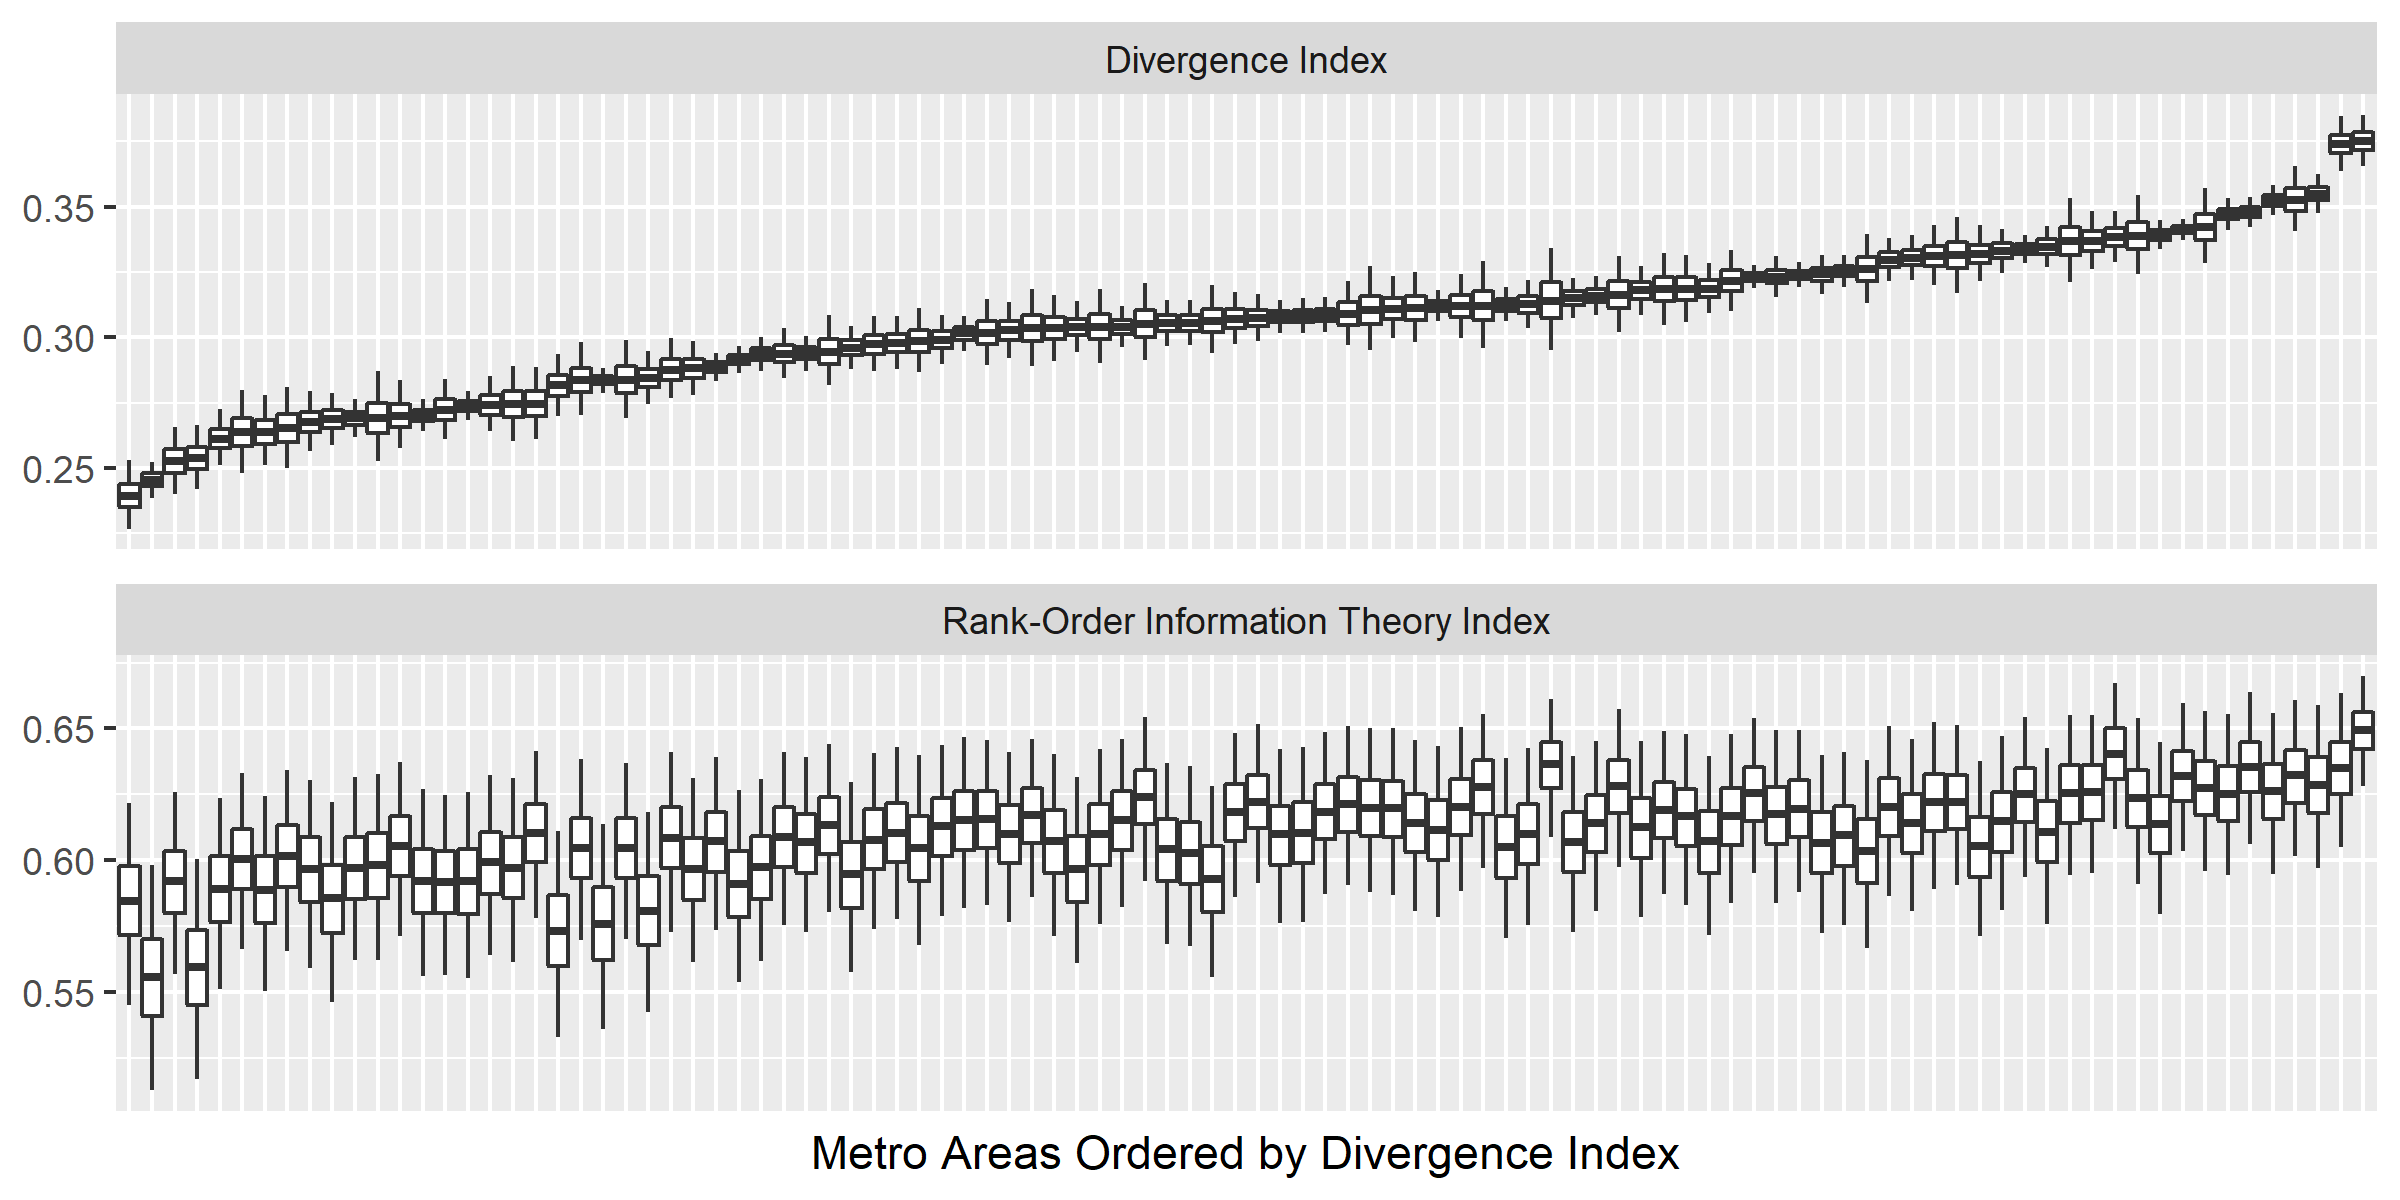
\includegraphics[scale = 0.9]{index_plot_combined.png}
\caption{Divergence index vs. information theory index for all households. Box plots represent the $2.5$, $25$, $50$, $75$, and $97.5$ percentiles of the posterior distribution of the index.}
\label{fig:indexplot}
\end{figure}

\begin{figure}[ht]
\centering
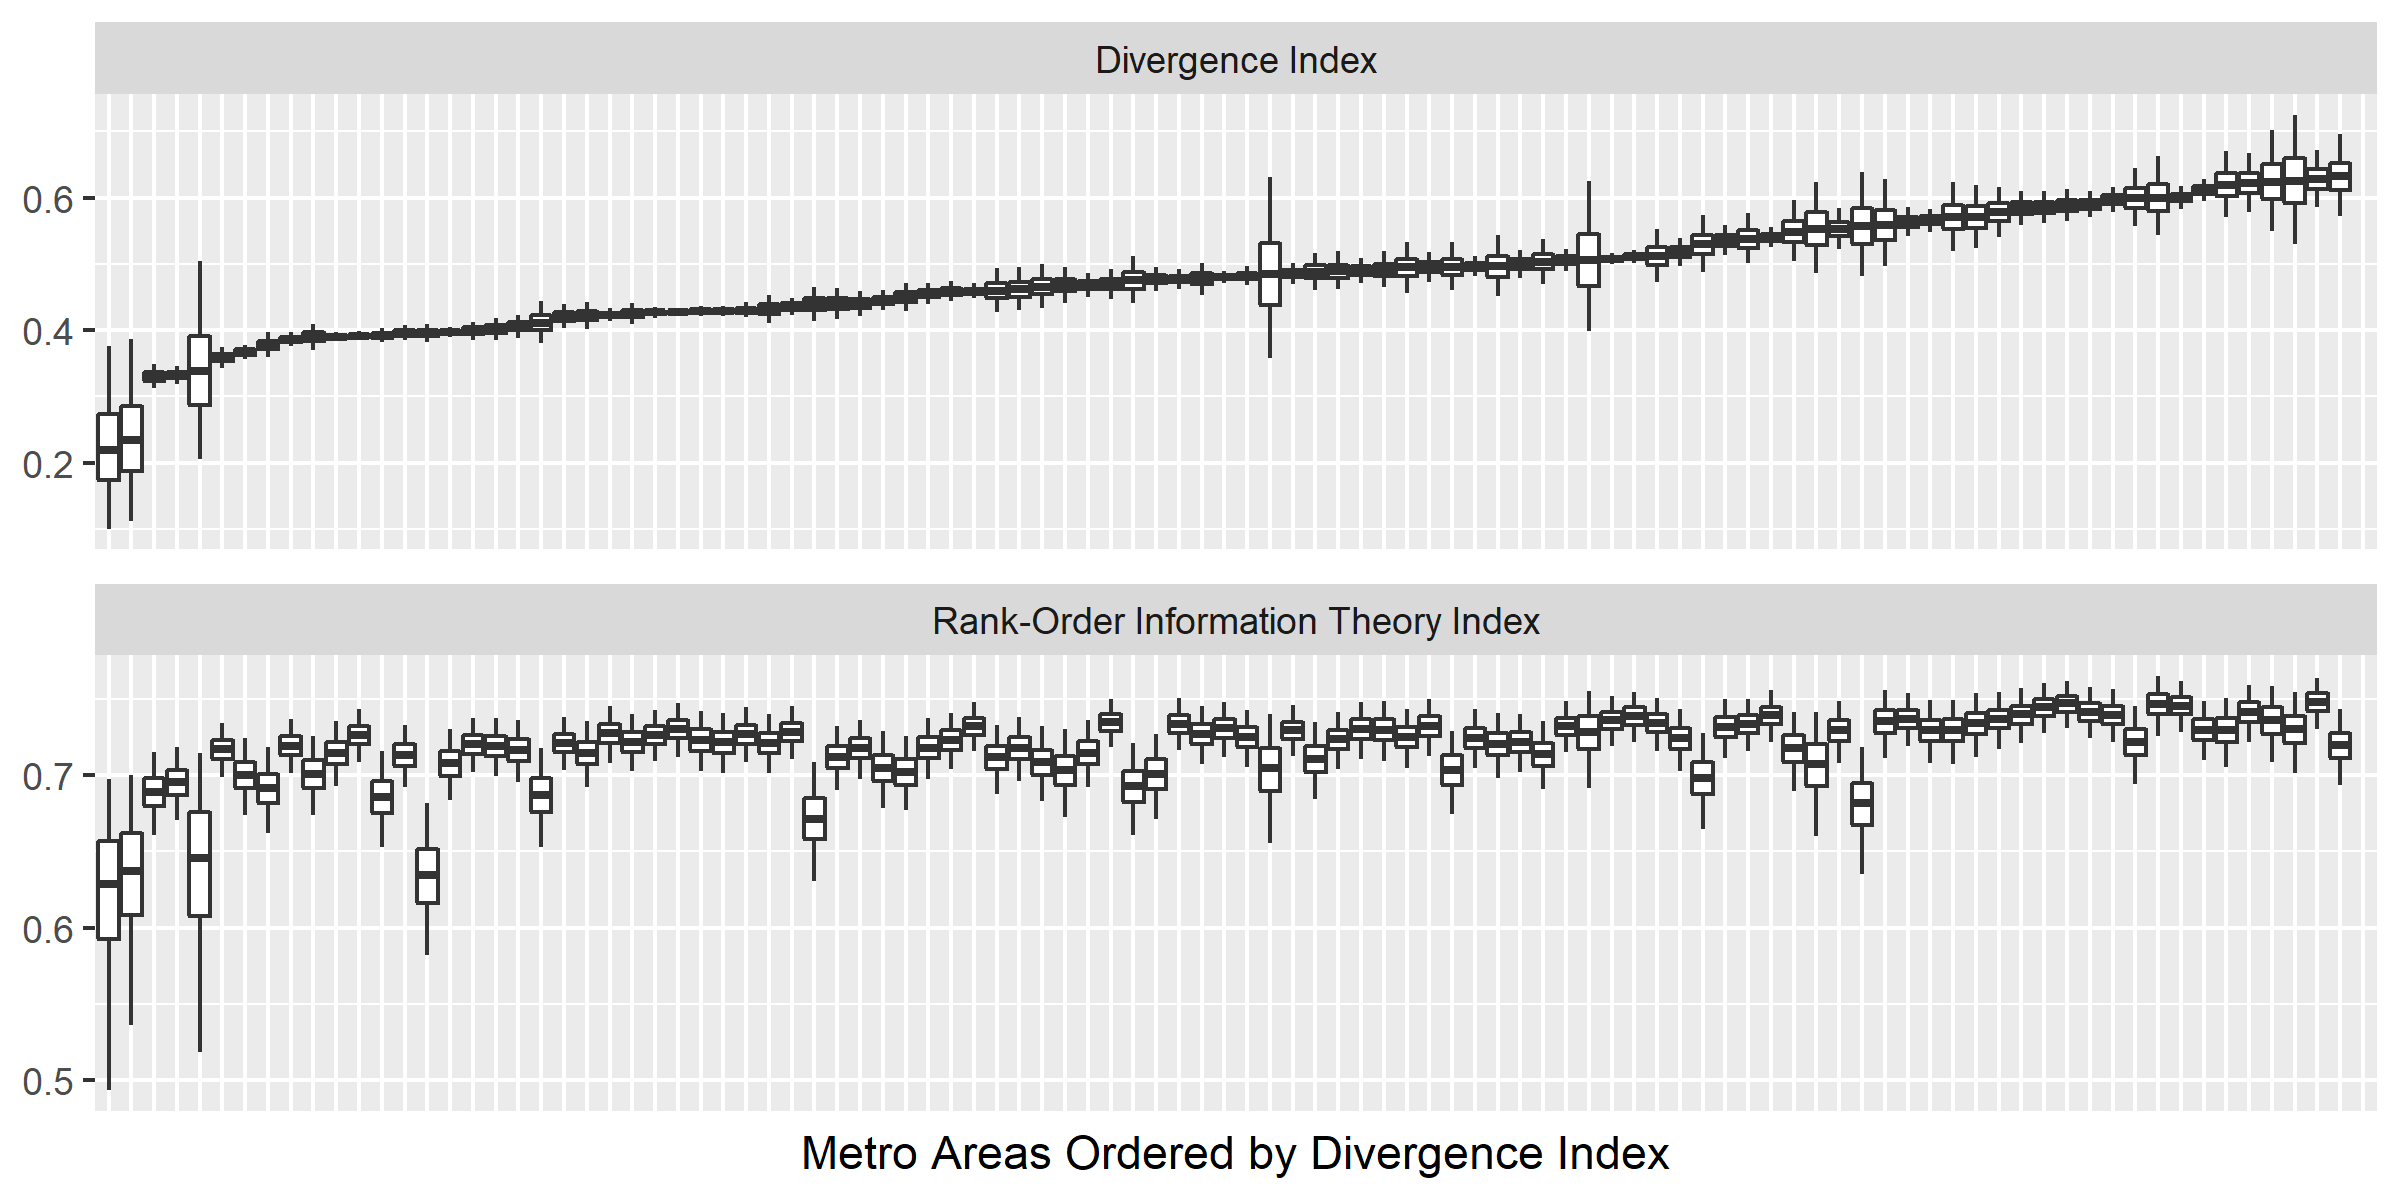
\includegraphics[scale = 0.9]{index_plot_black.png}
\caption{Divergence index vs. information theory index for black households. Box plots represent the $2.5$, $25$, $50$, $75$, and $97.5$ percentiles of the posterior distribution of the index.}
\label{fig:blackindexplot}
\end{figure}

\begin{figure}[ht]
\centering
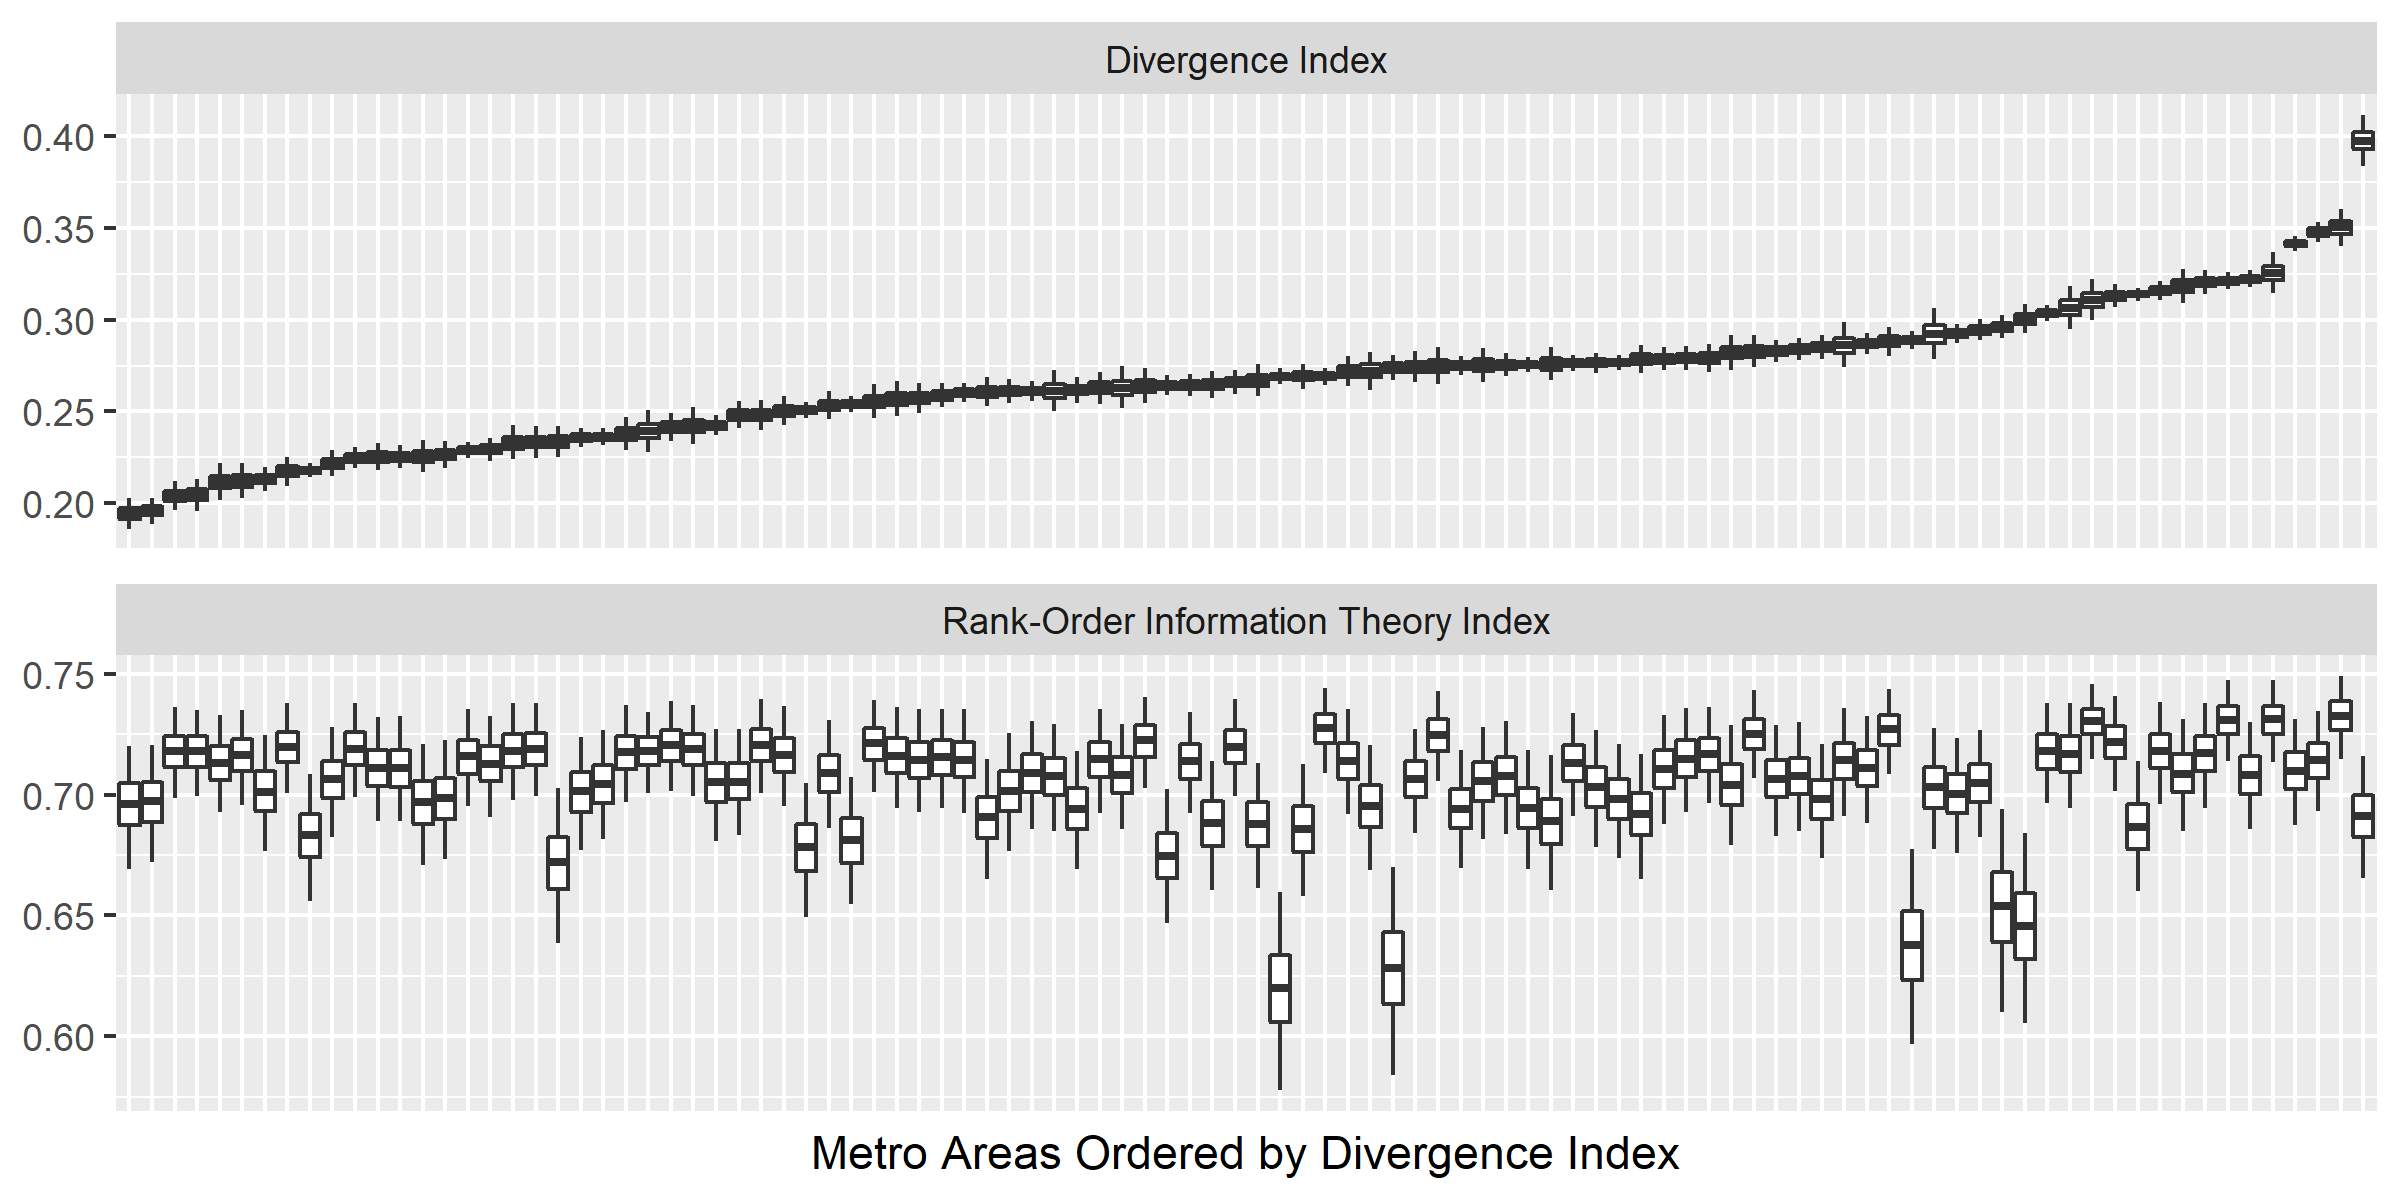
\includegraphics[scale = 0.9]{index_plot_white.png}
\caption{Divergence index vs. information theory index for white households. Box plots represent the $2.5$, $25$, $50$, $75$, and $97.5$ percentiles of the posterior distribution of the index.}
\label{fig:whiteindexplot}
\end{figure}

\clearpage
\subsection{Information Theory Index Regressions}

% latex table generated in R 4.0.3 by xtable 1.8-4 package
% Thu Dec 17 18:50:17 2020
\begin{table}[ht]
\centering
\begin{tabular}{rrrrrrrrr}
  \hline
 & OLS & Mean & SD & 2.5\% & 25\% & 50\% & 75\% & 97.5\% \\ 
  \hline
  Intercept & 0.304 & 0.237 & 0.087 & 0.068 & 0.177 & 0.236 & 0.296 & 0.406 \\ 
  Gini & 0.454 & 0.427 & 0.058 & 0.313 & 0.389 & 0.427 & 0.467 & 0.540 \\ 
  Population & 1.4E-09 & 1.2E-09 & 2.6E-10 & 7.0E-10 & 1.0E-09 & 1.2E-09 & 1.4E-09 & 1.7E-09 \\ 
  Unemp & 0.004 & 0.041 & 0.097 & -0.153 & -0.025 & 0.042 & 0.108 & 0.227 \\ 
  Edu & -0.031 & -0.010 & 0.043 & -0.095 & -0.038 & -0.010 & 0.019 & 0.073 \\ 
  Income & -1.5E-03 & -1.4E-03 & 2.6E-04 & -1.9E-03 & -1.6E-03 & -1.4E-03 & -1.2E-03 & -9.0E-04 \\ 
  AgeOver65 & -0.094 & -0.104 & 0.053 & -0.208 & -0.138 & -0.104 & -0.068 & -0.000 \\ 
  AgeUnder18 & -0.218 & -0.210 & 0.059 & -0.328 & -0.250 & -0.210 & -0.169 & -0.095 \\ 
  Foreign & -0.033 & -0.032 & 0.015 & -0.061 & -0.042 & -0.032 & -0.022 & -0.002 \\ 
  IndustyConstruct & 0.296 & 0.391 & 0.122 & 0.156 & 0.307 & 0.391 & 0.472 & 0.629 \\ 
  IndustryManuf & 0.080 & 0.085 & 0.041 & 0.005 & 0.058 & 0.085 & 0.113 & 0.165 \\ 
  IndustryFIRE & 0.028 & 0.046 & 0.046 & -0.045 & 0.016 & 0.046 & 0.077 & 0.136 \\ 
  IndustryProf & 0.077 & 0.067 & 0.036 & -0.002 & 0.043 & 0.068 & 0.091 & 0.138 \\ 
  FemaleHHer & 0.159 & 0.204 & 0.051 & 0.104 & 0.169 & 0.203 & 0.238 & 0.305 \\ 
  SameHouse & 0.087 & 0.122 & 0.067 & -0.009 & 0.077 & 0.121 & 0.168 & 0.253 \\ 
  SameCounty & 0.234 & 0.266 & 0.087 & 0.098 & 0.206 & 0.266 & 0.325 & 0.438 \\ 
  NewHouse & -0.135 & -0.122 & 0.111 & -0.337 & -0.198 & -0.124 & -0.045 & 0.096 \\ 
   \hline
\end{tabular}
\caption{OLS estimates and posterior summaries of EIV regression coefficients for the information theory index using all households.}
\label{tab:eiv.hr.raw.all}
\end{table}

% latex table generated in R 4.0.3 by xtable 1.8-4 package
% Thu Dec 17 18:50:19 2020
\begin{table}[ht]
\centering
\begin{tabular}{rrrrrrrrr}
  \hline
 & OLS & Mean & SD & 2.5\% & 25\% & 50\% & 75\% & 97.5\% \\ 
  \hline
Intercept & 0.817 & 0.730 & 0.191 & 0.346 & 0.611 & 0.729 & 0.848 & 1.119 \\ 
  Gini & -0.191 & -0.079 & 0.125 & -0.328 & -0.161 & -0.078 & 0.004 & 0.164 \\ 
  Population & -4.6E-09 & -4.4E-09 & 3.1E-09 & -1.1E-08 & -6.5E-09 & -4.4E-09 & -2.3E-09 & 1.7E-09 \\ 
  Unemp & -0.227 & -0.203 & 0.099 & -0.398 & -0.270 & -0.203 & -0.138 & -0.009 \\ 
  Edu & 0.011 & 0.077 & 0.053 & -0.027 & 0.041 & 0.077 & 0.112 & 0.180 \\ 
  Income & 1.6E-03 & 1.4E-04 & 7.7E-03 & -1.7E-02 & -3.5E-03 & 2.1E-04 & 3.8E-03 & 1.7E-02 \\ 
  AgeOver65 & -0.066 & -0.097 & 0.129 & -0.352 & -0.184 & -0.097 & -0.009 & 0.156 \\ 
  AgeUnder18 & -0.089 & -0.005 & 0.190 & -0.381 & -0.133 & -0.005 & 0.123 & 0.367 \\ 
  Foreign & 0.045 & 0.071 & 0.025 & 0.022 & 0.055 & 0.071 & 0.088 & 0.121 \\ 
  IndustyConstruct & -0.054 & -0.189 & 0.225 & -0.628 & -0.339 & -0.190 & -0.041 & 0.263 \\ 
  IndustryManuf & -0.058 & -0.037 & 0.064 & -0.160 & -0.079 & -0.037 & 0.006 & 0.089 \\ 
  IndustryFIRE & 0.142 & 0.144 & 0.088 & -0.032 & 0.085 & 0.144 & 0.203 & 0.318 \\ 
  IndustryProf & -0.063 & -0.037 & 0.052 & -0.138 & -0.073 & -0.038 & -0.003 & 0.066 \\ 
  SameHouse & 0.053 & 0.038 & 0.127 & -0.214 & -0.046 & 0.038 & 0.123 & 0.288 \\ 
  SameCounty & -0.068 & -0.255 & 0.194 & -0.632 & -0.384 & -0.256 & -0.124 & 0.124 \\ 
  NewHouse & 0.021 & 0.259 & 0.243 & -0.223 & 0.096 & 0.263 & 0.424 & 0.728 \\ 
   \hline
\end{tabular}
\caption{OLS estimates and posterior summaries of EIV regression coefficients for the information theory index using only black households.}
\label{tab:eiv.hr.raw.black}
\end{table}

% latex table generated in R 4.0.3 by xtable 1.8-4 package
% Thu Dec 17 18:50:19 2020
\begin{table}[ht]
\centering
\begin{tabular}{rrrrrrrrr}
  \hline
 & OLS & Mean & SD & 2.5\% & 25\% & 50\% & 75\% & 97.5\% \\ 
  \hline
Intercept & 0.682 & 0.955 & 0.230 & 0.491 & 0.813 & 0.956 & 1.098 & 1.415 \\ 
  Gini & 0.370 & 0.145 & 0.111 & -0.072 & 0.071 & 0.146 & 0.220 & 0.366 \\ 
  Population & 1.6E-09 & 2.0E-09 & 9.6E-10 & 1.3E-10 & 1.4E-09 & 2.0E-09 & 2.7E-09 & 3.9E-09 \\ 
  Unemp & -0.203 & 0.157 & 0.231 & -0.296 & 0.003 & 0.156 & 0.311 & 0.611 \\ 
  Edu & -0.021 & -0.243 & 0.060 & -0.361 & -0.283 & -0.242 & -0.202 & -0.124 \\ 
  Income & -2.5E-03 & 7.0E-05 & 5.5E-03 & -1.1E-02 & -3.0E-03 & -8.9E-05 & 3.1E-03 & 1.2E-02 \\ 
  AgeOver65 & -0.152 & 0.008 & 0.073 & -0.137 & -0.041 & 0.008 & 0.056 & 0.153 \\ 
  AgeUnder18 & -0.387 & -0.254 & 0.094 & -0.438 & -0.317 & -0.255 & -0.193 & -0.069 \\ 
  Foreign & -0.057 & -0.154 & 0.026 & -0.205 & -0.171 & -0.154 & -0.137 & -0.104 \\ 
  IndustyConstruct & 0.178 & -0.226 & 0.212 & -0.641 & -0.369 & -0.226 & -0.085 & 0.190 \\ 
  IndustryManuf & 0.004 & -0.177 & 0.063 & -0.299 & -0.220 & -0.178 & -0.136 & -0.054 \\ 
  IndustryFIRE & 0.083 & -0.008 & 0.080 & -0.166 & -0.062 & -0.008 & 0.045 & 0.149 \\ 
  IndustryProf & -0.017 & -0.215 & 0.055 & -0.321 & -0.252 & -0.215 & -0.179 & -0.106 \\ 
  SameHouse & 0.058 & 0.060 & 0.129 & -0.194 & -0.026 & 0.060 & 0.146 & 0.312 \\ 
  SameCounty & 0.246 & 0.557 & 0.174 & 0.218 & 0.441 & 0.558 & 0.673 & 0.897 \\ 
  NewHouse & -0.151 & 0.044 & 0.199 & -0.347 & -0.088 & 0.044 & 0.177 & 0.434 \\ 
   \hline
\end{tabular}
\caption{OLS estimates and posterior summaries of EIV regression coefficients for the information index using only white households.}
\label{tab:eiv.hr.raw.white}
\end{table}

\clearpage

\subsection{Divergence Index Regressions}

% latex table generated in R 4.0.3 by xtable 1.8-4 package
% Thu Dec 17 18:54:44 2020
\begin{table}[ht]
\centering
\begin{tabular}{rrrrrrrrr}
  \hline
 & OLS & Mean & SD & 2.5\% & 25\% & 50\% & 75\% & 97.5\% \\ 
  \hline
Intercept & -0.123 & -0.149 & 0.230 & -0.609 & -0.299 & -0.150 & -0.000 & 0.315 \\ 
  Gini & 0.765 & 0.763 & 0.157 & 0.458 & 0.657 & 0.762 & 0.868 & 1.074 \\ 
  Population & 2.9E-09 & 2.9E-09 & 9.0E-10 & 1.1E-09 & 2.3E-09 & 2.9E-09 & 3.5E-09 & 4.6E-09 \\ 
  Unemp & 0.508 & 0.496 & 0.292 & -0.067 & 0.298 & 0.496 & 0.688 & 1.068 \\ 
  Edu & -0.009 & -0.025 & 0.114 & -0.253 & -0.101 & -0.025 & 0.052 & 0.197 \\ 
  Income & -7.1E-04 & -6.8E-04 & 7.7E-04 & -2.2E-03 & -1.2E-03 & -6.8E-04 & -1.6E-04 & 8.2E-04 \\ 
  AgeOver65 & -0.243 & -0.232 & 0.131 & -0.484 & -0.321 & -0.232 & -0.145 & 0.023 \\ 
  AgeUnder18 & 0.048 & 0.053 & 0.153 & -0.252 & -0.050 & 0.053 & 0.157 & 0.351 \\ 
  Foreign & -0.088 & -0.090 & 0.051 & -0.191 & -0.125 & -0.091 & -0.056 & 0.009 \\ 
  IndustyConstruct & 0.341 & 0.410 & 0.330 & -0.232 & 0.194 & 0.404 & 0.629 & 1.061 \\ 
  IndustryManuf & 0.074 & 0.084 & 0.108 & -0.125 & 0.011 & 0.082 & 0.157 & 0.296 \\ 
  IndustryFIRE & 0.063 & 0.066 & 0.120 & -0.171 & -0.013 & 0.064 & 0.147 & 0.304 \\ 
  IndustryProf & 0.050 & 0.062 & 0.095 & -0.124 & -0.000 & 0.063 & 0.125 & 0.246 \\ 
  FemaleHHer & 0.122 & 0.152 & 0.133 & -0.119 & 0.065 & 0.151 & 0.240 & 0.406 \\ 
  SameHouse & -0.049 & -0.038 & 0.188 & -0.407 & -0.163 & -0.036 & 0.086 & 0.336 \\ 
  SameCounty & 0.464 & 0.512 & 0.259 & -0.012 & 0.341 & 0.513 & 0.685 & 1.020 \\ 
  NewHouse & -0.584 & -0.581 & 0.305 & -1.185 & -0.785 & -0.579 & -0.376 & 0.015 \\ 
   \hline
\end{tabular}
\caption{OLS estimates and posterior summaries of EIV regression coefficients for the divergence index using all households.}
\label{tab:eiv.kl.raw.all}
\end{table}

% latex table generated in R 4.0.3 by xtable 1.8-4 package
% Thu Dec 17 18:54:44 2020
\begin{table}[ht]
\centering
\begin{tabular}{rrrrrrrrr}
  \hline
 & OLS & Mean & SD & 2.5\% & 25\% & 50\% & 75\% & 97.5\% \\ 
  \hline
Intercept & -0.297 & -0.416 & 1.033 & -2.484 & -1.082 & -0.409 & 0.254 & 1.618 \\ 
  Gini & 0.699 & 1.403 & 0.742 & -0.036 & 0.899 & 1.402 & 1.898 & 2.872 \\ 
  Population & -6.2E-08 & -5.8E-08 & 1.6E-08 & -9.0E-08 & -6.9E-08 & -5.8E-08 & -4.8E-08 & -2.7E-08 \\ 
  Unemp & -1.156 & -1.545 & 0.531 & -2.584 & -1.902 & -1.546 & -1.195 & -0.485 \\ 
  Edu & 0.564 & 0.387 & 0.256 & -0.118 & 0.216 & 0.388 & 0.559 & 0.894 \\ 
  Income & -4.3E-03 & -2.6E-03 & 4.2E-02 & -8.8E-02 & -2.8E-02 & -4.5E-03 & 2.3E-02 & 8.6E-02 \\ 
  AgeOver65 & 0.037 & 0.214 & 0.508 & -0.773 & -0.128 & 0.210 & 0.551 & 1.220 \\ 
  AgeUnder18 & -0.153 & -0.009 & 0.809 & -1.602 & -0.550 & -0.014 & 0.530 & 1.596 \\ 
  Foreign & 0.459 & 0.402 & 0.118 & 0.166 & 0.323 & 0.403 & 0.480 & 0.633 \\ 
  IndustyConstruct & -0.046 & -0.475 & 1.131 & -2.711 & -1.233 & -0.473 & 0.288 & 1.722 \\ 
  IndustryManuf & 0.313 & 0.195 & 0.315 & -0.424 & -0.016 & 0.197 & 0.406 & 0.819 \\ 
  IndustryFIRE & 0.330 & 0.380 & 0.402 & -0.404 & 0.107 & 0.381 & 0.649 & 1.168 \\ 
  IndustryProf & 0.228 & 0.044 & 0.271 & -0.483 & -0.136 & 0.043 & 0.225 & 0.578 \\ 
  SameHouse & -0.049 & -0.084 & 0.647 & -1.346 & -0.519 & -0.086 & 0.348 & 1.198 \\ 
  SameCounty & 0.079 & 0.258 & 0.944 & -1.595 & -0.371 & 0.254 & 0.889 & 2.122 \\ 
  NewHouse & 0.533 & 0.556 & 1.098 & -1.619 & -0.169 & 0.557 & 1.286 & 2.723 \\ 
   \hline
\end{tabular}
\caption{OLS estimates and posterior summaries of EIV regression coefficients for the divergence index using black households only.}
\label{tab:eiv.kl.raw.black}
\end{table}

% latex table generated in R 4.0.3 by xtable 1.8-4 package
% Thu Dec 17 18:54:45 2020
\begin{table}[ht]
\centering
\begin{tabular}{rrrrrrrrr}
  \hline
 & OLS & Mean & SD & 2.5\% & 25\% & 50\% & 75\% & 97.5\% \\ 
  \hline
Intercept & 0.405 & 0.188 & 0.440 & -0.660 & -0.101 & 0.179 & 0.471 & 1.079 \\ 
  Gini & 0.489 & 0.683 & 0.240 & 0.207 & 0.523 & 0.683 & 0.843 & 1.155 \\ 
  Population & 4.5E-09 & 4.3E-09 & 2.1E-09 & 1.4E-10 & 2.9E-09 & 4.3E-09 & 5.7E-09 & 8.4E-09 \\ 
  Unemp & 0.473 & 0.356 & 0.497 & -0.630 & 0.024 & 0.356 & 0.690 & 1.326 \\ 
  Edu & -0.098 & -0.001 & 0.127 & -0.251 & -0.087 & -0.001 & 0.084 & 0.247 \\ 
  Income & 1.2E-03 & 1.4E-03 & 9.6E-03 & -1.9E-02 & -4.4E-03 & 2.5E-03 & 7.1E-03 & 2.0E-02 \\ 
  AgeOver65 & -0.567 & -0.638 & 0.154 & -0.939 & -0.741 & -0.638 & -0.535 & -0.338 \\ 
  AgeUnder18 & -0.091 & -0.146 & 0.197 & -0.531 & -0.279 & -0.146 & -0.014 & 0.239 \\ 
  Foreign & -0.039 & 0.002 & 0.055 & -0.107 & -0.035 & 0.002 & 0.039 & 0.112 \\ 
  IndustyConstruct & 0.286 & 0.530 & 0.458 & -0.374 & 0.225 & 0.531 & 0.835 & 1.429 \\ 
  IndustryManuf & -0.205 & -0.104 & 0.134 & -0.366 & -0.195 & -0.104 & -0.014 & 0.159 \\ 
  IndustryFIRE & -0.071 & -0.020 & 0.168 & -0.350 & -0.131 & -0.020 & 0.093 & 0.307 \\ 
  IndustryProf & -0.158 & -0.049 & 0.118 & -0.281 & -0.128 & -0.049 & 0.029 & 0.182 \\ 
  SameHouse & -0.200 & -0.215 & 0.277 & -0.760 & -0.400 & -0.217 & -0.031 & 0.327 \\ 
  SameCounty & 0.077 & -0.067 & 0.377 & -0.806 & -0.320 & -0.069 & 0.185 & 0.675 \\ 
  NewHouse & -0.381 & -0.492 & 0.432 & -1.347 & -0.775 & -0.491 & -0.207 & 0.352 \\ 
   \hline
\end{tabular}
\caption{OLS estimates and posterior summaries of EIV regression coefficients for the divergence index using white households only.}
\label{tab:eiv.kl.raw.white}
\end{table}

\clearpage

\subsection{Standardized Information Index Regression Coefficients}
\citet{reardon2011income} report raw information index regression coefficients in their Table~4. To be able to directly compare these coefficients to our own, especially our divergence index regression coefficients, we need to standardize them. To do this, we need the sample standard deviations of the information theory index and the Gini coefficient from the sample used for the regressions in \citet{reardon2011income}'s Table~4. They report basic summary statistics for each year-race cross section in their Table~2, which we can use to construct the combined-years sample standard deviations needed to standardize the coefficients in Table~4.

For a particular variable (information index or Gini coefficient) and a particular race (black, white, or all), we can construct the combined sample standard deviation as follows. Let $N$ denote the sample size for that variable per year---for white families and all families $N=100$, while for black families $N=61$. Additionally, let $k=1,2,...,K$ index years, $m_k$ denote the sample mean for year $k$, and $s_k$ denote the sample standard deviation for year $k$. First let
\begin{align*}
m = \frac{1}{K}\sum_{k=1}^Km_k
\end{align*}
denote the combined mean. Then the combined variance is given by
\begin{align*}
s^2= \frac{\sum_{k=1}^K\left[(N-1)s_k^2 + nm_k^2\right] - KNm^2}{KN - 1}
\end{align*}
and then combined standard deviation is given by $s = \sqrt{s^2}$.

Table~\ref{tab:sds} contains means and standard deviations for the Gini coefficient and the information index from \citet{reardon2011income}'s Table~2, as well as the combined standard deviations computed with the formula above.
Finally, Table~\ref{tab:std.coefs} contains the original raw from \citet{reardon2011income}'s Table~4 as well as the standardized coefficients using the combined standard deviations computed above.

\begin{table}[ht]
  \centering
  \begin{tabular}{l|rrrr|rrrrl}
& \multicolumn{4}{c}{Gini Coefficient Means} & \multicolumn{5}{c}{Gini Coefficient SDs} \\\hline
    Race  & 1970  & 1980  & 1990  & 2000  & 1970  & 1980  & 1990  & 2000  & Combined \\\hline
    All   & 0.352 & 0.360 & 0.384 & 0.400 & 0.029 & 0.023 & 0.026 & 0.025 & 0.032 \\    
    Black & 0.376 & 0.410 & 0.430 & 0.436 & 0.018 & 0.017 & 0.030 & 0.024 & 0.033 \\
    White & 0.344 & 0.341 & 0.369 & 0.384 & 0.028 & 0.020 & 0.026 & 0.025 & 0.031 \\
    \multicolumn{10}{c}{} \\
& \multicolumn{4}{c}{Information Index Means} & \multicolumn{5}{c}{Information Index SDs} \\\hline
    All   & 0.124 & 0.134 & 0.152 & 0.157 & 0.142 & 0.044 & 0.052 & 0.050 & 0.051 \\    
    Black & 0.099 & 0.133 & 0.173 & 0.170 & 0.144 & 0.029 & 0.036 & 0.042 & 0.049 \\
    White & 0.110 & 0.117 & 0.132 & 0.139 & 0.125 & 0.039 & 0.043 & 0.043 & 0.044 \\
  \end{tabular}
\label{tab:sds}
\caption{Means and standard deviations for the Gini coefficient and the information index from \citet{reardon2011income}.}
\end{table}


\begin{table}[ht]
  \centering
  \begin{tabular}{lrrrr}
      & \multicolumn{2}{c}{Raw $\widehat{\beta}$} & \multicolumn{2}{c}{Std $\widehat{\beta}$}\\\hline
    Race  & Beta & SE & Beta & SE \\\hline
    All   & 0.561 & 0.085 & 0.353 & 0.053 \\    
    Black & 0.470 & 0.124 & 0.316 & 0.083 \\
    White & 0.450 & 0.110 & 0.311 & 0.076 \\
  \end{tabular}
  \label{tab:std.coefs}
  \caption{Raw and standardized coefficients of the Gini coefficient from information index regressions from \citet{reardon2011income}.}
\end{table}

\clearpage

\bibliographystyle{jasa}  % (uses file "jasa.bst")
\bibliography{lprln}

\end{document} 

